% -*- Mode:TeX -*-

%% IMPORTANT: The official thesis specifications are available at:
%%            http://libraries.mit.edu/archives/thesis-specs/
%%
%%            Please verify your thesis' formatting and copyright
%%            assignment before submission.  If you notice any
%%            discrepancies between these templates and the 
%%            MIT Libraries' specs, please let us know
%%            by e-mailing thesis@mit.edu

%% The documentclass options along with the pagestyle can be used to generate
%% a technical report, a draft copy, or a regular thesis.  You may need to
%% re-specify the pagestyle after you \include  cover.tex.  For more
%% information, see the first few lines of mitthesis.cls. 

%\documentclass[12pt,vi,twoside]{mitthesis}
%%
%%  If you want your thesis copyright to you instead of MIT, use the
%%  ``vi'' option, as above.
%%
%\documentclass[12pt,twoside,leftblank]{mitthesis}
%%
%% If you want blank pages before new chapters to be labelled ``This
%% Page Intentionally Left Blank'', use the ``leftblank'' option, as
%% above. 

\documentclass[12pt,twoside]{mitthesis}
\usepackage{lgrind}
\usepackage{hyperref}
\usepackage{graphicx}
\usepackage{enumitem}
\usepackage{adjustbox}
\usepackage{multicol}
\usepackage{amssymb}
\usepackage{amsmath}
\usepackage{algorithm}
\usepackage[noend]{algpseudocode}
%% These have been added at the request of the MIT Libraries, because
%% some PDF conversions mess up the ligatures.  -LB, 1/22/2014
\usepackage{cmap}
\usepackage[T1]{fontenc}
\pagestyle{plain}

%% This bit allows you to either specify onwly the files which you wish to
%% process, or `all' to process all files which you \include.
%% Krishna Sethuraman (1990).

%\typein [\files]{Enter file names to process, (chap1,chap2 ...), or `all' to
%process all files:}
\def\all{all}
%\ifx\files\all \typeout{Including all files.} \else \typeout{Including only \files.} \includeonly{\files} \fi

\begin{document}
% -*-latex-*-
% 
% For questions, comments, concerns or complaints:
% thesis@mit.edu
% 
%
% $Log: cover.tex,v $
% Revision 1.8  2008/05/13 15:02:15  jdreed
% Degree month is June, not May.  Added note about prevdegrees.
% Arthur Smith's title updated
%
% Revision 1.7  2001/02/08 18:53:16  boojum
% changed some \newpages to \cleardoublepages
%
% Revision 1.6  1999/10/21 14:49:31  boojum
% changed comment referring to documentstyle
%
% Revision 1.5  1999/10/21 14:39:04  boojum
% *** empty log message ***
%
% Revision 1.4  1997/04/18  17:54:10  othomas
% added page numbers on abstract and cover, and made 1 abstract
% page the default rather than 2.  (anne hunter tells me this
% is the new institute standard.)
%
% Revision 1.4  1997/04/18  17:54:10  othomas
% added page numbers on abstract and cover, and made 1 abstract
% page the default rather than 2.  (anne hunter tells me this
% is the new institute standard.)
%
% Revision 1.3  93/05/17  17:06:29  starflt
% Added acknowledgements section (suggested by tompalka)
% 
% Revision 1.2  92/04/22  13:13:13  epeisach
% Fixes for 1991 course 6 requirements
% Phrase "and to grant others the right to do so" has been added to 
% permission clause
% Second copy of abstract is not counted as separate pages so numbering works
% out
% 
% Revision 1.1  92/04/22  13:08:20  epeisach

% NOTE:
% These templates make an effort to conform to the MIT Thesis specifications,
% however the specifications can change.  We recommend that you verify the
% layout of your title page with your thesis advisor and/or the MIT 
% Libraries before printing your final copy.
\title{Extensions to Behavioral Genetic Programming}

\author{Steven B. Fine}
% If you wish to list your previous degrees on the cover page, use the 
% previous degrees command:
%       \prevdegrees{A.A., Harvard University (1985)}
% You can use the \\ command to list multiple previous degrees
%       \prevdegrees{B.S., University of California (1978) \\
%                    S.M., Massachusetts Institute of Technology (1981)}
\prevdegrees{S.B., Massachusetts Institute of Technology (2016)}
\department{Department of Electrical Engineering and Computer Science}

% If the thesis is for two degrees simultaneously, list them both
% separated by \and like this:
% \degree{Doctor of Philosophy \and Master of Science}
\degree{Master of Engineering in Electrical Engineering and Computer Science}

% As of the 2007-08 academic year, valid degree months are September, 
% February, or June.  The default is June.
\degreemonth{February}
\degreeyear{2017}
\thesisdate{February 2, 2017}

%% By default, the thesis will be copyrighted to MIT.  If you need to copyright
%% the thesis to yourself, just specify the `vi' documentclass option.  If for
%% some reason you want to exactly specify the copyright notice text, you can
%% use the \copyrightnoticetext command.  
%\copyrightnoticetext{\copyright IBM, 1990.  Do not open till Xmas.}

% If there is more than one supervisor, use the \supervisor command
% once for each.
\supervisor{Una-May O'Reilly}{Principal Research Scientist, MIT CSAIL}

% This is the department committee chairman, not the thesis committee
% chairman.  You should replace this with your Department's Committee
% Chairman.
\chairman{Christopher J. Terman}{Chairman, Master of Engineering Thesis Committee}

% Make the titlepage based on the above information.  If you need
% something special and can't use the standard form, you can specify
% the exact text of the titlepage yourself.  Put it in a titlepage
% environment and leave blank lines where you want vertical space.
% The spaces will be adjusted to fill the entire page.  The dotted
% lines for the signatures are made with the \signature command.
\maketitle

% The abstractpage environment sets up everything on the page except
% the text itself.  The title and other header material are put at the
% top of the page, and the supervisors are listed at the bottom.  A
% new page is begun both before and after.  Of course, an abstract may
% be more than one page itself.  If you need more control over the
% format of the page, you can use the abstract environment, which puts
% the word "Abstract" at the beginning and single spaces its text.

%% You can either \input (*not* \include) your abstract file, or you can put
%% the text of the abstract directly between the \begin{abstractpage} and
%% \end{abstractpage} commands.

% First copy: start a new page, and save the page number.
\cleardoublepage
% Uncomment the next line if you do NOT want a page number on your
% abstract and acknowledgments pages.
% \pagestyle{empty}
\setcounter{savepage}{\thepage}
\begin{abstractpage}
% !TeX spellcheck = en_US

\begin{abstract}
ABSTRACT GOES HERE.
\vspace{1.5in}


\end{abstract}

\end{abstractpage}

% Additional copy: start a new page, and reset the page number.  This way,
% the second copy of the abstract is not counted as separate pages.
% Uncomment the next 6 lines if you need two copies of the abstract
% page.
% \setcounter{page}{\thesavepage}
% \begin{abstractpage}
% % !TeX spellcheck = en_US

\begin{abstract}
ABSTRACT GOES HERE.
\vspace{1.5in}


\end{abstract}

% \end{abstractpage}

\cleardoublepage

\section*{Acknowledgments}

I would like to thank Una-May O'Reilly for all of her guidance throughout this research project.  Not only did she help me find a project that interested me, but our discussions were instrumental for the progression of my research.  I would also like to thank Krzysztof Krawiec for our discussion on possible extensions to behavioral genetic programming, and for answering my questions about the original implementation.  Finally, I would like to thank Erik Hemberg for all of the help he provided me in getting my experiments up and running on the CSAIL cloud, and for our discussions about my experimental results.

%%%%%%%%%%%%%%%%%%%%%%%%%%%%%%%%%%%%%%%%%%%%%%%%%%%%%%%%%%%%%%%%%%%%%%
% -*-latex-*-

% Some departments (e.g. 5) require an additional signature page.  See
% signature.tex for more information and uncomment the following line if
% applicable.
% \include{signature}
\pagestyle{plain}
  % -*- Mode:TeX -*-
%% This file simply contains the commands that actually generate the table of
%% contents and lists of figures and tables.  You can omit any or all of
%% these files by simply taking out the appropriate command.  For more
%% information on these files, see appendix C.3.3 of the LaTeX manual. 
\tableofcontents
\newpage
\listoffigures
\newpage
\listoftables


\chapter{Introduction}
\label{chap:intro}
Genetic programming (GP) is a subfield of Artificial Intelligence, in which the principles of evolution are employed in order to produce programs with desired functionality.  Each such program is defined by a set of genes, which can be mutated and swapped in a manner similar to reproduction in biological organisms.  A typical genetic programming algorithm will start with a population of initial programs, which are randomly generated.  Each successive iteration, a population of new programs is generated from the old population.  Finally, the best programs from the two populations are selected, and the process is repeated until a sufficiently good program is found.

The power of this technique is that the programmer does not need to guess at the structure of the desired program.  All the programmer needs is a method to generate new programs from old programs, and a fitness function by which to compare the performance of one program to another.  On the surface, this seems like a very promising method to produce arbitrarily complex programs, as long as the programmer has an understanding of the desired output.  However, in practice, the landscape of programs is enormous, and often times there are many local optima, which prevent evolving programs from achieving the desired functionality.

There are a variety of techniques and adaptations to the basic genetic programming methodology that attempt to exploit features of the evolutionary process to arrive at optimal solutions more quickly.  One such technique, designed by Krawiec et al. \cite{krawiec} attempts to utilize information about how to identify useful subprograms.  These subprograms are components of programs in the population that will help drive the evolutionary process, even if they are a part of a program that may not perform well on the specified task.  This technique is termed \textit{behavioral genetic programming} (BGP).  The vision of this work is that BGP is a paradigm rich with possible extensions to explore, many of which could give deeper insight into genetic programming methods.

This work focuses on replicating the results first achieved by Krawiec et al., and exploring various extensions to the BGP paradigm.  This work proceeds as follows. Chapter \ref{chap:relatedwork} discusses the basics of genetic programming, and the key ideas behind BGP.  Chapter \ref{chap:implementation} discusses my implementation of BGP with the added ability of running many different configurations that were not explored by Krawiec et al.  Chapter \ref{chap:experiments} discusses the experiments that are performed, and Chapter \ref{chap:conclusion} discusses my contributions and possible paths for future work.

\chapter{Related Work}
\label{chap:relatedwork}
\section{Basics of Genetic Programming}
\subsection{Program Representations}
As is stated in Chapter \ref{chap:intro}, Genetic programming is a general technique that can be applied to almost any task domain.  However, this work predominantly focuses on the task of symbolic regression.  Symbolic regression aims to find a mathematical expression that fits a given dataset.  Therefore the programs in which we are interested define mathematical expressions by combining a set of primitive operations.

Much of the time in genetic programming random segments of code are being removed, inserted, and swapped between different programs.  Therefore, it is important to have a program representation that is resilient to these types of operations.  As a result, it can be useful to avoid loops, and other types of statements that could result in programs that do not terminate.  For this reason, often times a tree structure is employed, where the internal nodes of the trees are functions, with the children as the arguments, and the leaves of the trees are terminals, such as variables and constants.

For the task of symbolic regression, the functions can be any set of primitive mathematical functions, while the terminals will typically be the features of the data set.

The tree in Figure \ref{figure:gp_tree} represents a simple program, which computes the mathematical function $f(x) = \ln(x1) + (x1 - x2)$.  Given a larger set of mathematical operations, it is possible to create arbitrarily complex mathematical expressions.

\noindent
\begin{figure}[h]
\centering
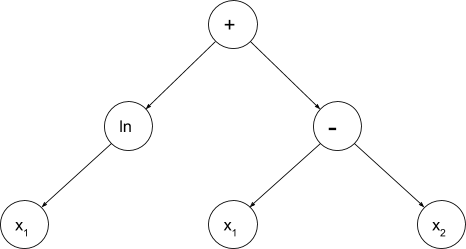
\includegraphics[width=110mm]{gp_tree_colorless}
\caption{Sample tree representing a program.}
\label{figure:gp_tree}
\end{figure}

\subsection{Generating New Programs}
\label{section:gp_operators}
One of the core aspects of genetic programming is how to generate a new population of programs from an old population.  There are two primary operations used to generate new programs: the mutation operation and the crossover operation.

\subsubsection{Mutation}
The mutation operation generates a single new program from a single old program.  First a mutation point is selected in the old program.  This can be selected uniformly at random, or biased towards certain parts of the tree.  Then the subtree located at the mutation point is removed, and a new subtree is generated in a similar way to how the first population of programs was generated.

\subsubsection{Crossover}
The crossover operation generates two new programs from two old programs.  First a crossover point is selected in each old program.  This can be done in any of the same ways that a mutation point is selected.  Then the subtrees located at the two crossover points in the two old programs are swapped, creating two new program trees.

\subsection{Choosing Programs to Survive}
After a new population of programs is generated, only half of the programs from the combined new and old populations are kept for the next generation of the evolutionary process.  If there is a single fitness function that is being optimized, this process is very straightforward.  Simply keep the programs that perform best on the fitness function.  However, often times there are multiple fitness functions that are used to drive the evolutionary process.  For example, in the case of symbolic regression, one fitness function could be the absolute error for predicting the dependent variable, while the other fitness function could be the program size.  When there are multiple fitness functions, often times one program will have a better fitness score than another program for one fitness function, but not the remaining fitness functions.  In this case a different method must be used to determine which programs should be kept.  The method used for the purpose of this work is discussed in section \ref{section:survival}.

\subsection{Termination}
The run of a genetic program terminates after one of several conditions is met.  The following are common termination conditions:
\begin{enumerate}[noitemsep]
\item An optimal program is found.
\item A maximum number of generations is reached.
\item The run has exceeded the maximum allocated amount of time.
\end{enumerate}

\section{Behavioral Genetic Programming}
One extension to the genetic programming paradigm is behavioral genetic programming (BGP) \cite{krawiec}.  As was mentioned in Chapter \ref{chap:intro}, BGP attempts to identify useful subprograms that can then be used to enhance the evolutionary process.

\subsection{Trace}
In most genetic programming algorithms, the search is driven by the output of the fitness functions alone.  Only programs that perform well on the fitness functions are kept, while the rest are rejected.  However, every subtree that makes up an individual program has a distinct numerical output for each fitness case in any given data set.

Let us consider the program in Figure \ref{figure:gp_tree}, and the sample data set in Table \ref{table:sample_data}.  Conventional genetic programming will only consider the outputs for each data point: $\ln(3) + 1$, $\ln(5) + 2$, and compare those values to the desired output.  However, each subtree has its own output, which is ignored by the genetic programming process.

\begin{table*}[ht]
\centering
\begin{tabular}{ c c | c }
\hline\hline
$x_{1}$ & $x_{2}$ & $y$ \\ [0.5ex]
\hline
3 & 2 & 3 \\
5 & 3 & 4 \\[1ex]
\hline
\end{tabular}
\caption{Sample data set.}
\label{table:sample_data}
\end{table*}

The collection of the outputs on each subtree for all of the data points is called the trace.  For the program in Figure \ref{figure:gp_tree} and the fitness cases in Table \ref{table:sample_data}, the trace is shown in Table \ref{table:sample_trace}.

\begin{table*}[ht]
\centering
\begin{tabular}{ c c c c c c }
\hline\hline
$s_{1}$ & $s_{2}$ & $s_{3}$ & $s_{4}$ & $s_{5}$ & $s_{6}$ \\ [0.5ex]
\hline
3 & $\ln(3)$ & 3 & 2 & 1 & $\ln(3)$ + 1 \\
5 & $\ln(5)$ & 5 & 3 & 2 & $\ln(5)$ + 2 \\[1ex]
\hline
\end{tabular}
\caption{The trace of the program from Figure \ref{figure:gp_tree} for the data set in Table \ref{table:sample_data}.}
\label{table:sample_trace}
\end{table*}

The trace is a matrix where the number of rows is equal to the number of data points, and the number of columns is equal to the number of subtrees in a given program.  There is no set order of the columns, although here they are presented in the depth first traversal order of the subtrees that produce the values.  The trace captures a full snapshot of all of the intermediate states of the program evaluation.

\subsection{Model}
The key idea behind Behavioral Programming is to exploit the trace to identify useful subtrees.  Ordinary crossover does not incorporate any information about the quality of the subtrees that are being swapped.  However, the trace opens up many possibilities to explore the quality of subtrees.  In Behavioral Programming, the trace is used to train a machine learning model to predict the desired output for each fitness case.  The model is then used for two purposes.  The first is to create additional fitness measures by which to evaluate a given program.  The second is to identify useful subtrees based on the composition of this model, which are then placed in an archive.  The content of the archive is then used for the supply the subtrees that are used in the crossover operation, instead of taking arbitrary subtrees from other programs in the population.



\chapter{Implementation}
\label{chap:implementation}

The following section details my implementation of behavioral genetic programming.  It follows the details  presented by Krawiec et al. \cite{krawiec}, with several adaptions in order to explore several variants of BGP.

\section{Codebase}
The codebase that I use for this project was first built for FlexGP \cite{flexgp} and then extended for the implementation of Multiple Regression Genetic Programming (MRGP) \cite{mrgp}.  It is written in the Java programming language.  With simple modifications the codebase could run conventional GP for symbolic regression tasks.  One of the main contributions of my work is the way in which I extended the codebase.  Many of the abstractions that I introduced allow the GP process to be extended in unforeseen ways.

\section{Genetic Programming Run}
During the execution of a genetic programming algorithm, there are three steps associated with any given generation.  The steps are as follows:

\begin{itemize}[noitemsep]
\item \textbf{Initialization/Reproduction}: Generate a new population of programs.  In the first round of evolution, the programs are generated from scratch.  In all subsequent rounds the programs are generated from the programs in the old population.
\item \textbf{Evaluation}: Evaluate all of the programs in the new population.
\item \textbf{Survival}: Select which programs in the combined population will be kept for the next round of evolutionary computation.
\end{itemize}

\subsection{Initialization}
When the GP run is initialized, the first step is to create an initial population of programs.  The number of programs in each generation is specified by the user at the start of the run.  The programs are generated by randomly choosing functions and terminals as children of the parent nodes, until every leaf in the tree is a terminal.  A maximum depth is specified, and the trees are generated such that the trees vary from having a depth of one to the maximum depth.

\subsection{Reproduction}
In all subsequent generations, new programs are generated from the population of programs belonging to the previous generation.  One of the modifications that I made was the introduction of a reproduction operator.  Previously the mutation operator and crossover operator were hardcoded as the only possible operators used to generate new children.  The reproduction operator introduces a method to add children to the new population, which can have many different implementations.  For the purposes of this work, the implementation of the reproduction operator that is used allows mutation, crossover, and archive-based crossover, each with an associated probability of being used, each time new programs are to be generated.  This implementation enables the use of conventional GP by setting the archive-based crossover probability to zero.

\subsubsection{Selection of Programs for Reproduction}
During reproduction, new programs are generated until the population size is reached.  To generate a new program, an old program (or in case of crossover, a pair of old programs) is selected to have one of the reproduction operators applied.  The process by which a program is selected is called \textit{tournament selection}.  A tournament size is specified in the parameters of the GP run.  For a given tournament size $n$, $n$ individuals are drawn uniformly at random from the population, and then compete to determine which individual will have the reproduction operator applied.  The winner of the competition is simply the program with the highest rank based on the NSGA-II algorithm \cite{nsga}.  The NSGA-II algorithm is discussed in Section \ref{section:survival}.

\subsubsection{Reproduction Operators}
The mutation and crossover operations were discussed in Section \ref{section:gp_operators}.  In the implementation of behavioral genetic programming by Krawiec et al., the mutation and crossover points for a given program tree are selected by first choosing the depth of the point uniformly at random from 1 to the depth of the tree, then choosing a node uniformly at random from the given depth.  The third operation, archive-based crossover, works identically to the mutation operator, with the exception of how the new subtrees are generated.  In ordinary mutation, the subtrees are generated in the same manner that each member of the initial population of programs is generated.  However, in archive-based crossover, the subtrees are drawn from an archive, which maintains a weighted distribution over which subtrees will be selected.  The archive is discussed further in section \ref{section:evaluation}.

\subsection{Evaluation}
\label{section:evaluation}
Once a new population of programs is generated, all of the new programs must be evaluated on all of the fitness functions that are being used for the genetic programming run.  Additionally, in the case of behavioral genetic programming, the archive is populated based on a machine learning model that is generated from the trace of each program.  This section details the process by which these steps are accomplished.

\subsubsection{Fitness Function Evaluation}
Another abstraction that I introduced into the codebase is that of a fitness function evaluator.  In conventional genetic programming, the program fitness functions can be evaluated in any order, and all that is needed is the numerical output for each fitness function for each program.  In behavioral genetic programming there are two classes of fitness functions.  The functions in the first class only require the programs themselves to be evaluated.  The fitness functions in conventional genetic programming belong to this class.  The functions in the second class require a machine learning model built on the trace of each program to be evaluated.  For each possible configuration of BGP, a different fitness function evaluator is used, which takes care of the proper order for the fitness functions to be evaluated, and the generation of the model.  The different configurations are discussed in Section \ref{section:setup} and detailed in Appendix \ref{appendix:configuration_parameters}.

%\subsubsection{Fitness Functions}
\subsubsection{Conventional Genetic Programming Fitness Functions}
\label{section:conventional_fitness_functions}
In conventional genetic programming, there are typically two fitness functions used to evaluate a program.  The first is the program error $f$, which is a measure of how close the program output on each data point is to the desired output.  The form of the program error fitness used by Krawiec et al. is given by Equation \ref{eq:program_error}, where $\hat y$ is the output of the program, $y$ is the desired output, and $d_{m}$ denotes the Manhattan distance between the two arguments.  The second fitness function is typically a measure of program size $s$, where smaller programs are considered more fit than larger programs.  The form of the program size fitness used by Krawiec et al. is given by Equation \ref{eq:program_size}, where $|p|$ is the number of nodes in the tree that defines the program.

\begin{equation}
\label{eq:program_error}
f = 1 - \frac{1}{1 + d_{m}(\hat y, y)}
\end{equation}

\begin{equation}
\label{eq:program_size}
s = 1 - \frac{1}{|p|}
\end{equation}

\subsubsection{Behavioral Genetic Programming Fitness Functions}
In behavioral genetic programming there are four fitness functions.  Two are the conventional fitness functions discussed in Section \ref{section:conventional_fitness_functions}.  The remaining fitness functions that are used are the model complexity $c$, given by Equation \ref{eq:model_complexity}, and the model error $e$, given by Equation \ref{eq:model_error}, where $M$ is the output of the machine learning model when it is evaluated on the trace of the program, and $|M|$ is the size of the model.

%The model is discussed further in Section \ref{section:model}.

One of the most expensive operations in the execution of a genetic program is the evaluation of each program on all of the data points.  This step is required for both calculating the program error fitness, and generating the trace of the program.  Therefore, in behavioral genetic programming, the trace for a given program is generated while the program error fitness value is calculated.

\begin{equation}
\label{eq:model_complexity}
c = 1 - \frac{1}{|M|}
\end{equation}

\begin{equation}
\label{eq:model_error}
e = 1 - \frac{1}{1 + d_{m}(M, y)}
\end{equation}

\subsubsection{Model}
\label{section:model}
Once the trace for a given program in the population has been collected the machine learning model can be built.  The purpose of the model is two-fold.  The first is that it introduces additional fitness measures for each program (given by Equations \ref{eq:model_complexity} and \ref{eq:model_error}).  Second, it guides the process of populating the archive.

The algorithm that was used for the model in the original implementation of behavioral genetic programming, by Krawiec et al. was REPTree. \cite{reptree}  REPTree is a decision tree that can be used for both classification and regression tasks.  For each program in the population, a different model is built on the program trace.  In my implementation, one can use different models by writing different implementations for the model interface.

\subsubsection{Archive}
In behavioral genetic programming, an archive is used from which to draw subtrees that are used for archive-based crossover.  The archive is given a maximum capacity, which in the original implementation of Behavioral Programming by Krawiec et al. was set to 50.  After each round of fitness function evaluations, the archive is repopulated in the following way.  First the candidate subtrees are selected based on whether or not their column in the trace was used in the machine learning model.  Each subtree is assigned a weight given by Equation \ref{eq:subtree_weight}, where $e$ is the model error from Equation \ref{eq:model_error} and $|U|$ is the number of distinct columns of the trace used in the model.  Note that all subtrees that are used in a certain model are given the same weight in the archive.  Each generation, after the model has been generated, the candidate subtrees are combined with the pre existing contents of the archive (with the exception of the first generation, as the archive would be empty).  If the number of candidate subtrees combined with the previous contents of the archive is less than the archive capacity, then all of the subtrees are added to the archive.  If the number of candidate subtrees combined with the previous contents of the archive is greater than the capacity of the archive, then subtrees are drawn without replacement with probability proportional to their assigned weights.  Algorithm \ref{pseudocode} illustrates this procedure.  For my implementation I use a modification \cite{samplingnew} of the algorithm introduced by Efraimidis and Spirakis \cite{samplingold} to efficiently draw from a weighted distribution without replacement (Note that Algorithm \ref{pseudocode} does not include the details of this procedure).  When subtrees are drawn from the archive for archive-based crossover, they are drawn from the weighted distribution with replacement.

\begin{equation}
\label{eq:subtree_weight}
w = \frac{1}{(1 + e)|U|}
\end{equation}

\begin{algorithm}
\caption{Populate Archive}\label{pseudocode}
\begin{algorithmic}[1]
\Procedure{PopulateArchive}{}
\For {\textit{subtree}\text{ in }\textit{archive}}
\State $w \gets \text{the weight of }\textit{subtree}$
\State $\text{add (}\textit{subtree,w}\text{) to }\textit{candidateSubtrees}$
\EndFor
\State $\text{clear }\textit{archive}$
\For {\textit{program}\text{ in }\textit{population}}
\State $T \gets \textit{collectTrace(program)}$
\State $\textit{M} \gets \textit{buildModel(T)}$
\State $U \gets \text{subtrees included in } \textit{M}$
\State $w \gets 1/((1 + e)|U|)$
\For {\textit{subtree}\text{ in }\textit{U}}
\State $\text{add (}\textit{subtree,w}\text{) to }\textit{candidateSubtrees}$
\EndFor
%\State $\text{add }$\text{(}\textit{U, w}\text{)}\text{ to }\textit{candidateSubtrees}
\EndFor
\If {|\textit{candidateSubtrees}| $\leq$ \textit{ARCHIVE\_CAPACITY}}
\State $\text{add all }\textit{candidateSubtrees}\text{ to }\textit{archive}$
\Else
\While {\textit{archive.size} $<$ \textit{ARCHIVE\_CAPACITY}}
\State $\textit{subtree} \gets \text{draw from }\textit{candidateSubtrees}$
\State $w \gets \text{the weight of }\textit{subtree}$
\State $\text{remove (}\textit{subtree,w}\text{) from }\textit{candidateSubtrees}$
\State $\text{add (}\textit{subtree,w}\text{) to }\textit{archive}$
\EndWhile
\EndIf
\EndProcedure
\end{algorithmic}
\end{algorithm}

One significant implementation detail is that the archive cannot have two subtrees which both have the same output on all of the data points (termed the same \textit{semantics}).  In both the original implementation and my own, if two subtrees have the same semantics, then only the subtree with fewer nodes is kept.  Subtrees are duplicated both when they are added to the archive, and drawn from the archive, to ensure that no two programs have a reference to the same subtree.

\subsection{Survival}
\label{section:survival}
Once all of the fitness functions have been evaluated, and the archive repopulated, only half of the programs from the combination of the old and new generation may be kept.  Given that in conventional genetic programming and behavioral genetic programming there are multiple fitness functions, we cannot simply keep the programs that perform best on the fitness functions.  Many programs may perform well on one metric, at the expense of another.  Therefore the NSGA-II algorithm \cite{nsga} is used to rank all of the programs in the combined population, and only the highest ranking half of the combined population is kept for the next generation.

The NSGA-II algorithm first classifies each program into a series of fronts.  The first front (termed \textit{pareto front}) is defined by all of the programs for which no other program in the population performs better on at least one fitness function, and as well or better on the remaining fitness functions.  Each successive front is defined by first removing the last front from the population, and recomputing the next front on the remaining programs in the same way that the pareto front was computed.  Every program in a given front outranks all programs in all subsequent fronts, and is outranked by all programs in all previous fronts.

Within a given front each program is ranked by its crowding distance.  To compute the crowding distance of an individual program, first all fitness measures are normalized (Note that in BGP we use fitness functions which are already normalized).  Then for each fitness measure, the difference between the fitness of the program with the next highest fitness and the next lowest fitness is computed.  The crowding distance for an individual program is given by the average difference across all fitness measures.  If for a given fitness measure an individual program has either the highest or lowest fitness value in the population, it receives a crowding distance of infinity.  Programs with higher crowding distances outrank programs with lower crowding distances.  The reason for the crowding distance ranking is to increase the diversity of the population.  Programs with higher crowding distances are more dissimilar to other programs in the population.

\section{Extensions to Behavioral Genetic Programming}
\label{section:extensions}
One of the core goals of this work is to explore different extensions and alternative implementations of behavioral genetic programming.  For the purpose of this work I explore several variants of the BGP machine learning model, which are detailed below.

\subsection{Full Population Model}
One of the main ideas that I explore is how the model would perform if instead of training one model on the trace of each program in the population, I train one model for the entire population on the combined traces of all of the programs.  This effectively creates a single trace matrix with the same number of rows but many more columns.  The combined trace matrix represents an extremely high dimensional problem, with uninvestigated correlation of its features.

The idea behind training a model for each individual in the population is twofold.  The first is that the accuracy of the model gives insight into how much information the subtrees in a program encode about the desired output. The second is that knowing which subtrees are used in the model gives insight into which subtrees are more valuable than others.  What it does not tell us is which subtrees will work well with other subtrees in the population.

The motivation behind combining all of the program traces to train a single machine learning model is to hopefully identify groups of subtrees coming from different programs in the population that work well together.  With this method one can populate the archive in the same way as in ordinary BGP, however, one cannot use the additional fitness measures, because each program in the population does not have a distinct model error and model complexity associated with it.

\subsection{Lasso Model}
Another implementation that I explore uses Least Absolute Shrinkage and Selection Operator (Lasso) as the machine learning model.  Instead of training REPTree on the trace of each program in the population, I run the Lasso regression method.  For each feature in the data set on which Lasso is run, it assigns a real valued weight.  The predicted output is given by the inner product of the features in the data set, and the weights assigned by Lasso, plus a real valued offset.  One benefit to Lasso is that it will perform feature selection by assigning some feature weights a value of 0.  In this model, I use the same formula for model error, and I define the size of the model $|M|$ as the number of features with non-zero coefficients.  Only subtrees with corresponding features that are given non-zero weights by Lasso are included in the archive.  I use the absolute value of the weights assigned by Lasso as the weight for each respective subtree in the archive.

\subsection{Scikit Learn Model}
Another implementation of the model interface that I employ uses the Python Scikit Learn DecisionTreeRegressor class for regression.  This model works identically to the model that uses REPTree with the exception of calling an alternative implementation of a decision tree.

\subsection{Randomized Model}
Finally, I use an implementation that is identical to the model used in REPTree, however, for each subtree used in the resulting REPTree decision tree, before being placed in the archive, it is replaced by a subtree drawn uniformly at random from the subtrees in the program.  The purpose of this implementation is not to see whether or not this model performs better than the model that uses the subtrees from REPTree.  Rather, it is used to illuminate how much is gained from populating the archive with the trees that are used by REPTree.

\chapter{Experiments}
\label{chap:experiments}

\section{Setup}
\label{section:setup}
In order to test the performance of different behavioral genetic programming models, I run 16 distinct configurations of BGP on the same 17 data sets that are used for the task of symbolic regression by Krawiec et al.  The basis of the data sets is taken from a paper entitled \textit{Genetic Programming Needs Better Benchmarks} by McDermott et al. \cite{benchmarks} The complete specification of all 17 data sets is presented in Appendix \ref{appendix:data_sets}.

The basis of the 16 BGP configurations that I use, comes from the 3 BGP configurations used by Krawiec et al.:

\begin{enumerate}[noitemsep]
\item \textbf{BP2A} uses only the program error fitness function and the program size fitness function (Equations \ref{eq:program_error} and \ref{eq:program_size}), but replaces crossover with archive-based crossover.
\item \textbf{BP4} uses all four BGP fitness functions (Equations \ref{eq:program_error}, \ref{eq:program_size}, \ref{eq:model_complexity}, and \ref{eq:model_error}), but performs ordinary crossover.
\item \textbf{BP4A} uses all four BGP fitness functions, and replaces crossover with archive-based crossover.
\end{enumerate}

%I use a population size of 100 programs, a mutation rate of $0.1$, and a crossover rate of $0.9$.  The mutation rate and crossover rate are the relative probability that each operation is used.  Each run terminates after 250 generations.

Note that in all three variants, the same model is constructed.  The only distinction is for what the model is used.  In addition to running the three configurations above using the REPTree model (as is done by Krawiec et al.), I run each of the three configurations using each of the models specified in Section \ref{section:extensions}.  I also explore several other parameter configurations. I explore the use of a larger archive, and the use of different mutation and archive-based crossover rates.  Specifically, in several runs I use a mutation rate of $0.05$, and a archive-based crossover rate of $0.95$.  The reason for this last variant is that GP crossover creates two new programs each time it is called.  However, archive-based crossover only creates one new program.  These altered operation rates closely simulate the creation of two new programs each time archive-based crossover is called.

For a baseline comparison, I run conventional GP with the two conventional GP fitness functions described in Section \ref{section:evaluation}.  For all of the runs, I use the same parameters that are specified by Krawiec et al.  A complete list of the parameters that are fixed for every run can be found in Appendix \ref{appendix:fixed_parameters}.  The following is a complete list of the 17 configurations (16 BGP, 1 conventional GP) that I run.  Their exact specifications are detailed in Appendix \ref{appendix:configuration_parameters}.

\begin{multicols}{2}
\begin{enumerate}
\item GP
\item BP2A - REPTree
\item BP2A - Full Pop
\item BP2A - Lasso
\item BP2A - Scikit Learn
\item BP2A - Randomized
\item BP2A - Larger Archive
\item BP2A - Different Rates
\item BP4 - REPTree
\item BP4 - Lasso
\item BP4 - Scikit Learn
%\item BP4 - Randomized
\item BP4A - REPTree
\item BP4A - Lasso
\item BP4A - Scikit Learn
\item BP4A - Randomized
\item BP4A - Larger Archive
\item BP4A - Different Rates
\end{enumerate}
\end{multicols}

For the majority of the configurations, I perform 30 runs on each data set.  However, all of the Scikit Learn configurations take much longer to run because they require calling Python from within Java.  Therefore, they are run 5 times each.  Additionally, BP2A - Lasso, and BP4A - Lasso, both did not run to completion.  As a result, they are omitted from the discussion.  They are addressed in Section \ref{section:future_work}.

\section{Results}
Appendix \ref{appendix:results} contains tables for the average and standard deviation of program fitness, program size, and program runtime, for the best of run programs for each configuration and data set.  A best of run program is the program with the lowest program error generated in a given run.  Additionally, there is a table with the percentage of runs that produced a perfect individual for each configuration and dataset.  Below I discuss the results in aggregate and compare them to those of Krawiec et al.

%\begin{table*}[ht]
\centering
\begin{adjustbox}{width=1\textwidth}
\small
\begin{tabular}{ c c c c c c c c c c c c c c c c c c c }
\hline\hline
 & & Keij1 & Keij11 & Keij12 & Keij13 & Keij14 & Keij15 & Keij4 & Keij5 & Nguy10 & Nguy12 & Nguy3 & Nguy4 & Nguy5 & Nguy6 & Nguy7 & Nguy9 & Sext \\
 \hline
GP &  & 0.338 & 0.858 & 0.97 & 0.562 & 0.798 & \textbf{0.87} & 0.6 & 0.989 & 0.106 & 0.38 & 0.181 & \textbf{0.247} & 0.108 & 0.017 & 0.114 & 0.1 & 0.102 \\
\hline
BP2A & REPTree & \textbf{0.243} & 0.776 & 0.972 & 0.393 & 0.723 & 0.883 & 0.384 & 0.975 & 0.11 & \textbf{0.343} & 0.196 & 0.265 & 0.037 & 0.091 & 0.122 & 0.068 & 0.052 \\
 & Full Pop & 0.272 & 0.864 & 0.982 & 0.565 & 0.809 & 0.947 & 0.397 & 0.977 & 0.304 & 0.393 & 0.376 & 0.372 & 0.081 & 0.277 & 0.179 & 0.214 & 0.129 \\
 & Scikit Learn & 0.327 & 0.769 & \textbf{0.966} & 0.481 & 0.726 & 0.907 & 0.468 & 0.977 & 0.199 & 0.379 & 0.2 & 0.285 & 0.04 & 0.119 & 0.127 & 0.075 & 0.054 \\
 & Randomized & 0.289 & 0.788 & 0.973 & 0.462 & 0.816 & 0.875 & 0.504 & 0.979 & 0.223 & 0.385 & 0.227 & 0.277 & \textbf{0.021} & 0.044 & 0.144 & 0.047 & 0.075 \\
 & Larger Archive & 0.286 & \textbf{0.566} & 0.97 & 0.388 & 0.742 & 0.877 & 0.397 & 0.977 & 0.146 & 0.344 & 0.192 & 0.257 & 0.029 & 0.112 & 0.127 & 0.059 & \textbf{0.051} \\
 & Different Rates & 0.272 & 0.694 & 0.976 & \textbf{0.326} & 0.773 & 0.882 & \textbf{0.37} & \textbf{0.974} & 0.165 & 0.361 & 0.202 & 0.284 & 0.031 & 0.071 & \textbf{0.103} & 0.042 & 0.054 \\
 \hline
BP4 & REPTree & 0.359 & 0.852 & 0.982 & 0.817 & 0.872 & 0.922 & 0.522 & 0.993 & 0.309 & 0.388 & 0.193 & 0.33 & 0.103 & 0.133 & 0.117 & 0.165 & 0.127 \\
 & Lasso & 0.324 & 0.833 & 0.985 & 0.669 & 0.811 & 0.916 & 0.511 & 0.987 & \textbf{0.105} & 0.365 & 0.292 & 0.399 & 0.13 & 0.08 & 0.182 & 0.103 & 0.092 \\
 & Scikit Learn & 0.357 & 0.684 & 0.968 & 0.548 & 0.776 & 0.887 & 0.513 & 0.991 & 0.144 & 0.36 & 0.266 & 0.288 & 0.126 & \textbf{0.0} & 0.104 & \textbf{0.04} & 0.083 \\
 \hline
BP4A & REPTree & 0.319 & 0.804 & 0.981 & 0.765 & 0.821 & 0.919 & 0.505 & 0.991 & 0.209 & 0.386 & 0.22 & 0.328 & 0.088 & 0.117 & 0.128 & 0.194 & 0.1 \\
 & Scikit Learn & 0.261 & 0.811 & 0.973 & 0.507 & \textbf{0.691} & 0.94 & 0.471 & 0.981 & 0.264 & 0.379 & 0.219 & 0.273 & 0.034 & 0.088 & 0.115 & 0.065 & 0.056 \\
 & Randomized & 0.338 & 0.844 & 0.984 & 0.705 & 0.844 & 0.939 & 0.56 & 0.989 & 0.338 & 0.414 & 0.197 & 0.364 & 0.104 & 0.137 & 0.138 & 0.145 & 0.118 \\
 & Larger Archive & 0.321 & 0.858 & 0.982 & 0.738 & 0.788 & 0.922 & 0.529 & 0.99 & 0.271 & 0.367 & 0.222 & 0.348 & 0.137 & 0.125 & 0.136 & 0.118 & 0.096 \\
 & Different Rates & 0.32 & 0.815 & 0.98 & 0.779 & 0.802 & 0.913 & 0.525 & 0.991 & 0.226 & 0.375 & \textbf{0.145} & 0.303 & 0.112 & 0.134 & 0.12 & 0.215 & 0.102 \\
\hline
\end{tabular}
\end{adjustbox}
\caption{Average program error for best of run programs.}
\label{table:avg_fitness}
\end{table*}



%\begin{table*}[ht]
%\centering
%\begin{adjustbox}{width=1\textwidth}
%\small
%\begin{tabular}{ c c c c c c c c c c c c c c c c c c c }
%\hline\hline
% & & Keij1 & Keij11 & Keij12 & Keij13 & Keij14 & Keij15 & Keij4 & Keij5 & Nguy10 & Nguy12 & Nguy3 & Nguy4 & Nguy5 & Nguy6 & Nguy7 & Nguy9 & Sext \\
% \hline
% GP & & 0.303 & 0.851 & 0.968 & 0.391 & 0.841 & 0.879 & 0.576 & 0.986 & 0.163 & 0.381 & 0.221 & 0.246 & 0.128 & \textbf{0.004} & \textbf{0.077} & 0.108 & 0.076 \\
% \hline
%BP2A & REPTree & 0.272 & 0.784 & 0.97 & \textbf{0.306} & 0.887 & 0.874 & \textbf{0.344} & 0.974 & 0.13 & 0.352 & 0.225 & 0.247 & 0.033 & 0.101 & 0.119 & 0.069 & 0.054 \\
%& Full Pop & 0.313 & 0.889 & 0.979 & 0.653 & 0.879 & 0.94 & 0.434 & 0.979 & 0.31 & 0.395 & 0.37 & 0.381 & 0.095 & 0.323 & 0.235 & 0.233 & 0.112 \\
%& Lasso & - & - & - & - & - & - & - & - & - & - & - & - & - & - & - & - & - \\
%& Scikit Learn & \textbf{0.22} & 0.876 & 0.98 & 0.45 & \textbf{0.753} & 0.88 & 0.411 & 0.984 & \textbf{0.091} & 0.379 & 0.187 & \textbf{0.204} & 0.043 & 0.046 & 0.151 & 0.076 & \textbf{0.037} \\
%& Randomized & 0.322 & 0.813 & 0.979 & 0.385 & 0.9 & 0.913 & 0.534 & 0.977 & 0.17 & 0.378 & 0.224 & 0.286 & \textbf{0.023} & 0.078 & 0.129 & 0.079 & 0.057 \\
%& Larger Archive & 0.278 & 0.719 & 0.975 & 0.434 & 0.893 & 0.889 & 0.405 & 0.983 & 0.165 & 0.35 & 0.196 & 0.287 & 0.024 & 0.089 & 0.151 & 0.09 & 0.044 \\
%& Different Rate & 0.266 & 0.725 & 0.979 & 0.311 & 0.894 & \textbf{0.867} & 0.374 & \textbf{0.969} & 0.152 & 0.354 & 0.191 & 0.263 & 0.025 & 0.055 & 0.117 & \textbf{0.064} & 0.041 \\
%\hline
%BP4 & REPTree & 0.467 & 0.908 & 0.989 & 0.914 & 0.916 & 0.915 & 0.706 & 0.997 & 0.412 & 0.444 & 0.222 & 0.327 & 0.275 & 0.086 & 0.113 & 0.201 & 0.26 \\
%& Lasso & - & - & - & - & - & - & - & - & - & - & - & - & - & - & - & - & - \\
%& Scikit Learn & 0.32 & \textbf{0.547} & \textbf{0.95} & 0.43 & 0.874 & 0.885 & 0.475 & 0.989 & 0.098 & 0.387 & 0.244 & 0.269 & 0.111 & 0.111 & 0.113 & 0.082 & 0.083 \\
%& Randomized & 0.468 & 0.855 & 0.989 & 0.902 & 0.92 & 0.919 & 0.694 & 0.997 & 0.428 & 0.437 & 0.253 & 0.366 & 0.253 & 0.073 & 0.139 & 0.186 & 0.201 \\
%\hline
%BP4A & REPTree & 0.435 & 0.912 & 0.988 & 0.891 & 0.92 & 0.909 & 0.672 & 0.997 & 0.37 & 0.438 & 0.206 & 0.352 & 0.152 & 0.154 & 0.132 & 0.221 & 0.217 \\
%& Lasso & - & - & - & - & - & - & - & - & - & - & - & - & - & - & - & - & - \\
%& Scikit Learn & 0.357 & 0.701 & 0.975 & 0.46 & 0.801 & 0.913 & 0.397 & 0.982 & 0.274 & \textbf{0.347} & 0.226 & 0.329 & 0.038 & 0.027 & 0.115 & 0.076 & 0.076 \\
%& Randomized & 0.471 & 0.92 & 0.989 & 0.874 & 0.923 & 0.938 & 0.706 & 0.997 & 0.404 & 0.432 & 0.239 & 0.334 & 0.201 & 0.119 & 0.105 & 0.196 & 0.154 \\
%& Larger Archive & 0.443 & 0.919 & 0.988 & 0.897 & 0.917 & 0.936 & 0.69 & 0.997 & 0.356 & 0.421 & 0.206 & 0.306 & 0.167 & 0.179 & 0.131 & 0.183 & 0.22 \\
%& Different Rate & 0.436 & 0.909 & 0.988 & 0.873 & 0.916 & 0.918 & 0.681 & 0.997 & 0.4 & 0.413 & \textbf{0.186} & 0.375 & 0.135 & 0.123 & 0.127 & 0.303 & 0.212 \\
%\hline
%\end{tabular}
%\end{adjustbox}
%\caption{Best of run individual fitness}
%\label{table:fitness}
%\end{table*}


Table \ref{table:ranks} contains the average rank for each configuration across all data sets for a variety of metrics.

%, and Table \ref{table:avg_fitness} contains the average program error for the best of run program for each configuration and data set.

\subsubsection{Average Rank for BGP with REPTree}
Krawiec et al found that the three BGP configurations that they run rank as follows for the given metrics:

\begin{itemize}[noitemsep]
\item \textbf{Program fitness}: BP4A, BP2A, BP4, GP
\item \textbf{Number of perfect programs found}: BP4A, BP2A, BP4, GP
\item \textbf{Program size}: GP, BP4, BP2A, BP4A
\item \textbf{Program runtime}: GP, BP4, BP4A, BP2A
\end{itemize}

It is important to note that the above ranks by Krawiec et al. are calculated based on the performance of each configuration across multiple task domains: boolean, categorical, and regression, while I only implement BGP for regression.  Both Krawiec et al., and I find that program fitness rank is inversely proportional to program size rank.  For program runtime, both sets of results suggest that GP is by far the fastest, and using an archive is slower than not.  For program fitness, both Krawiec et al., and I find that using an archive results in a better fitness than if an archive is not used, however, my results suggest that the added fitness functions hurt the evolutionary process.  Considering average fitness rank, it seems as though the BGP paradigm of replacing crossover with archive-based crossover is certainly beneficial.  However, considering the number of perfect programs found, my results suggest that configurations with an archive do not perform as well.

\begin{table*}[ht]
\centering
\begin{adjustbox}{width=1\textwidth}
\small
\begin{tabular}{ c | c c | c c }
\hline\hline
& Average Fitness Rank & & Average Rank For Finding Perfect Programs & \\
\hline
1 & BP2A - Different Rates & 3.53 & GP & 1.47 \\
2 & BP2A - REPTree & 4.06 & BP2A - Scikit Learn & 2.06 \\
3 & BP2A - Scikit Learn & 4.71 & BP4 - Scikit Learn & 2.06 \\
4 & GP & 5.35 & BP2A - Larger Archive & 2.59 \\
5 & BP2A - Larger Archive & 5.41 & BP2A - REPTree & 2.65 \\
6 & BP4A - Scikit Learn & 5.65 & BP4 - Lasso & 2.76 \\
7 & BP4 - Scikit Learn & 6.06 & BP2A - Randomized & 2.82 \\
8 & BP2A - Randomized & 6.18 & BP2A - Different Rates & 2.88 \\
9 & BP2A - Full Pop & 9.94 & BP4 - REPTree & 2.88 \\
10 & BP4 - Lasso & 10.88 & BP4A - Scikit Learn & 2.88 \\
11 & BP4A - Different Rates & 11.12 & BP4A - Larger Archive & 3.59 \\
12 & BP4A - REPTree & 11.53 & BP4A - Randomized & 3.65 \\
13 & BP4A - Larger Archive & 11.65 & BP4A - REPTree & 3.88 \\
14 & BP4 - REPTree & 11.88 & BP4A - Different Rates & 4.18 \\
15 & BP4A - Randomized & 12.06 & BP2A - Full Pop & 4.76 \\
\hline\hline
& Average Size Rank & & Average Runtime Rank & \\
 \hline
1 & BP4 - REPTree & 3.0 & GP & 1.0 \\
2 & BP4 - Lasso & 3.88 & BP4 - REPTree & 2.0 \\
3 & BP4 - Scikit Learn & 5.82 & BP2A - Different Rates & 3.24 \\
4 & BP4A - Randomized & 5.94 & BP4A - Larger Archive & 5.41 \\
5 & BP4A - REPTree & 6.35 & BP4A - Different Rates & 5.41 \\
6 & GP & 6.65 & BP2A - Larger Archive & 5.94 \\
7 & BP4A - Larger Archive & 7.06 & BP2A - Randomized & 6.47 \\
8 & BP4A - Different Rates & 7.29 & BP4A - Randomized & 7.76 \\
9 & BP2A - Scikit Learn & 9.41 & BP2A - REPTree & 8.82 \\
10 & BP2A - Different Rates & 9.41 & BP4A - REPTree & 9.18 \\
11 & BP4A - Scikit Learn & 9.53 & BP2A - Full Pop & 10.76 \\
12 & BP2A - Randomized & 10.0 & BP4 - Lasso & 12.18 \\
13 & BP2A - Larger Archive & 10.24 & BP2A - Scikit Learn & 13.29 \\
14 & BP2A - REPTree & 10.35 & BP4 - Scikit Learn & 13.94 \\
15 & BP2A - Full Pop & 14.88 & BP4A - Scikit Learn & 14.59 \\
\hline
\end{tabular}
\end{adjustbox}
\caption{Average rank of each configuration across all data sets.}
\label{table:ranks}
\end{table*}

%\begin{table*}[ht]
%\centering
%\begin{adjustbox}{width=1\textwidth}
%\small
%\begin{tabular}{ c | c c | c c }
%\hline\hline
%& Average Fitness Rank & & Average Rank For Finding Perfect Programs & \\
%\hline
%1 & BP2A - Different Rates & 3.53 & GP & 1.53 \\
%2 & BP2A - REPTree & 4.12 & BP2A - Scikit Learn & 2.12 \\
%3 & BP2A - Scikit Learn & 4.82 & BP4 - Scikit Learn & 2.18 \\
%4 & GP & 5.35 & BP2A - Larger Archive & 2.71 \\
%5 & BP2A - Larger Archive & 5.53 & BP2A - REPTree & 2.82 \\
%6 & BP4A - Scikit Learn & 5.65 & BP4 - Randomized & 2.88 \\
%7 & BP4 - Scikit Learn & 6.12 & BP2A - Randomized & 3.0 \\
%8 & BP2A - Randomized & 6.24 & BP2A - Different Rates & 3.0 \\
%9 & BP2A - Full Pop & 10.35 & BP4 - Lasso & 3.0 \\
%10 & BP4 - Lasso & 11.18 & BP4A - Scikit Learn & 3.0 \\
%11 & BP4A - Different Rates & 11.47 & BP4 - REPTree & 3.06 \\
%12 & BP4A - REPTree & 11.94 & BP4A - Larger Archive & 3.76 \\
%13 & BP4A - Larger Archive & 11.94 & BP4A - Randomized & 3.88 \\
%14 & BP4 - REPTree & 12.41 & BP4A - REPTree & 4.06 \\
%15 & BP4A - Randomized & 12.53 & BP4A - Different Rates & 4.47 \\
%16 & BP4 - Randomized & 12.82 & BP2A - Full Pop & 5.06 \\
%\hline\hline
%& Average Size Rank & & Average Runtime Rank & \\
% \hline
%1 & BP4 - Randomized & 3.0 & GP & 1.0 \\
%2 & BP4 - REPTree & 3.41 & BP4 - REPTree & 2.0 \\
%3 & BP4 - Lasso & 4.41 & BP4 - Randomized & 3.65 \\
%4 & BP4 - Scikit Learn & 6.53 & BP2A - Different Rates & 3.88 \\
%5 & BP4A - Randomized & 6.88 & BP4A - Larger Archive & 6.41 \\
%6 & BP4A - REPTree & 7.29 & BP4A - Different Rates & 6.41 \\
%7 & GP & 7.47 & BP2A - Larger Archive & 6.82 \\
%8 & BP4A - Larger Archive & 8.0 & BP2A - Randomized & 7.35 \\
%9 & BP4A - Different Rates & 8.29 & BP4A - Randomized & 8.76 \\
%10 & BP2A - Scikit Learn & 10.24 & BP2A - REPTree & 9.76 \\
%11 & BP2A - Different Rates & 10.41 & BP4A - REPTree & 10.18 \\
%12 & BP4A - Scikit Learn & 10.41 & BP2A - Full Pop & 11.76 \\
%13 & BP2A - Randomized & 11.0 & BP4 - Lasso & 13.18 \\
%14 & BP2A - Larger Archive & 11.24 & BP2A - Scikit Learn & 14.29 \\
%15 & BP2A - REPTree & 11.35 & BP4 - Scikit Learn & 14.94 \\
%16 & BP2A - Full Pop & 15.88 & BP4A - Scikit Learn & 15.59 \\
%\hline
%\end{tabular}
%\end{adjustbox}
%\caption{Average rank of each configuration across all data sets.}
%\label{table:ranks}
%\end{table*}

%\begin{table*}[ht]
%\centering
%\begin{adjustbox}{width=1\textwidth}
%\small
%\begin{tabular}{ c c c }
%\hline\hline
%& Average Fitness Rank & Average Rank For Finding Perfect Programs \\
%\hline
%1 & BP4A & BP4A \\
%2 & BP2A & BP2A \\
%3 & BP4 & BP4 \\
%4 & GP & GP \\
%\hline\hline
%& Average Size Rank & Average Runtime Rank \\
% \hline
%1 & GP & GP \\
%2 & BP4 & BP4 \\
%3 & BP2A & BP4A \\
%4 & BP4A & BP2A \\
%\hline
%\end{tabular}
%\end{adjustbox}
%\caption{Average rank of each configuration across all data sets.}
%\label{table:ranks}
%\end{table*}

\subsubsection{Full Population Model}
It seems that running the model on the each program trace is almost always better than running the model on the combined trace of the entire population.  In the full population case, each generation, the archive is only populated with subtrees taken from a single model, which might result in a less diverse archive.  Further work is needed to understand precisely why this model performs less well.

\subsubsection{Lasso Model}
The most significant feature of BGP that this configuration brings to light is that it is important to use a highly robust machine learning model for BGP.  Even for BP4 - Lasso, which did run to completion, the standard deviation of the runtimes are by far the largest (see Table \ref{table:std_time}).  The results also suggest, that for BP4, Lasso may provide better additional fitness measures than REPTree.

\subsubsection{Scikit Learn Model}
Because each BGP configuration using the Scikit Learn Model was only run five times on each data set, it is hard to make strong conclusions about its performance.  However, it seems that the resulting fitness is neither conclusively better nor worse than using REPTree.  However, the runtimes of all of the Scikit Learn Model configurations were notably the longest.  This is primarily due to the overhead of running a model that is written in the Python programming language, and calling it from Java.

\subsubsection{Randomized Model}
The randomized model consistently performed worse than the model that used the trees generated by REPTree.  This gives confidence to the claim that the subtrees generated by REPTree are more beneficial for driving the evolutionary process. 

\subsubsection{Larger Archive}
The results suggest that using a larger archive does not substantially help nor harm the resulting fitness of the generated programs.

\subsubsection{Different Rates}
It does appear that for both relevant BGP configurations, using a higher archive-based crossover rate, slightly improves the resulting program fitness for a given run.  This seems to invalidate the possibility that BGP only performed better than GP because the effective reproduction operator probabilities were substantially different from conventional GP.  It is also noteworthy, that using a higher archive-based crossover rate decreases the average runtime.



\chapter{Conclusion}
\label{chap:conclusion}

\section{Contributions} 
\label{section:contributions}
My primary contributions are threefold.

\begin{enumerate}[noitemsep]
\item Provide support for the claims of BGP by Krawiec et al.
\item Create a BGP implementation that is easily extendable for future work related to BGP.
\item Explore numerous extensions to and features of the BGP methodology.
\end{enumerate}

\section{Future Work}
\label{section:future_work}
A lot of what this work brings to light is particular paths to extend the concepts and understanding of BGP.  Below I detail several avenues to explore.

\subsubsection{Alternate Models}
The primary avenue that this work opens up is the possibility of exploring different models to use in BGP.  It would be interesting to see if using a machine learning model whose purpose is more inline with what BGP asks for would benefit the evolutionary process.  For example, instead of building an entire machine learning model on the trace, one could use a feature selection technique, or measure the statistical correlation between the columns.  The output would provide material with which to populate the archive.  However, this would not provide additional fitness measures.

\subsubsection{Lasso}
Lasso brought several interesting features of BGP to light.  It is important to have a machine learning model that is robust against the pathological inputs that can be generated by a genetic programming algorithm.  It would be interesting to explore why Lasso in general, or at least the implementation that I use has significant trouble for certain inputs.  Additionally, it is interesting that even though running Lasso is the runtime bottle neck, the configurations that took substantially too long to run were BP2A, and BP4A, both of which use an archive.  Understanding precisely why the configurations with an archive produce worse inputs to Lasso could be insightful.

\subsubsection{Mixing Traces}
It is unclear exactly why the BGP model that uses the combined traces of all of the programs in the population performed less well than running the model on each program trace independently.  It is possible that the idea has merit, but the particulars were not a good fit for BGP.  In particular, in each generation only a single machine learning model is built.  Therefore, all of the selected trees put into the archive in a single generation have the same weight.

An alternate implementation would be to draw random subsets from the combined trace of the programs in the population, and build a model on each.  This would create many candidate subtrees with different weights, and possibly a more robust archive, if it can be populated with subtrees that are frequently selected by the machine learning model.

\subsubsection{Subtrees with the Same Semantics}
As is mentioned in Section \ref{section:evaluation} if two subtrees have identical columns in the program trace (i.e. identical \textit{semantics}), only the smaller subtree is kept.  This introduces a bias that is not necessarily beneficial to the evolutionary process.  It would be interesting to explore how common subtrees with identical semantics are, and if choosing the smaller tree is the better choice.

\subsubsection{Combining Reproduction Operators}
It would be interesting to see if combining mutation, crossover, and archive-based crossover could enable better performance than using only two of the reproduction operators.

%% This subsubsection was the result of a bug in the implementation for FlexGP.  It should have been the sum of the fitness measure differents, not the product.  
%
%\subsubsection{Program Size and Model Complexity Fitness Functions}
%I find that for both the program size fitness function, and the model complexity fitness function, a lot of programs in the population have the same values as other programs in the population.  This frequently results in these programs having a crowding distance of zero.  It would be interesting to try using a fitness measure that has more diversity between programs in the population.  Alternatively, one could try out setting the minimum possible distance between two programs for a each fitness function as some $\epsilon$.  This would allow programs that have identical values for one fitness function to be compared relative to each other based on the diversity of the output of the other fitness functions.

%\subsubsection{Model Error}
%Comparing the performance of REPTree vs the Scikit Learn decision tree, I find that REPTree typically builds models with much higher errors when run on the trace, while Scikit Learn builds models with near zero error.  It would be interesting to explore what impact this has to the evolutionary process.

\subsubsection{Model Evaluation}
In BGP, after the model is built on the trace of each program, it is evaluated on the trace.  The result of its evaluation is used as the output of one of the fitness functions for the program.  It would be interesting to explore evaluating each model on a test set, instead of the trace.  Perhaps this would yield a more useful fitness function.

%\section{Conclusion}

\appendix
\chapter{Data Sets}
\label{appendix:data_sets}

All of the data sets used are defined such that the dependent variable is the output of a particular mathematical function for a given set of inputs.  They are taken from a paper entitled \textit{Genetic Programming Needs Better Benchmarks} by McDermott et al. \cite{benchmarks}  All of the inputs are taken to form a grid on some interval.  Let $E[a, b, c]$ denote $c$ samples equally spaced in the interval $[a,b]$. (Note that McDermott et al. defines $E[a, b, c]$ slightly differently.)  Below is a list of all of the data sets that are used:

\begin{enumerate}[noitemsep]
\item \textbf{Keijzer1}: $0.3x \sin(2 \pi x);$ $x \in E[-1,1,20]$
\item \textbf{Keijzer11}: $x y+\sin((x-1)(y-1));$ $x, y \in E[-3,3,5]$
\item \textbf{Keijzer12}: $x^{4}-x^{3}+\frac{y^{2}}{2}-y;$ $x, y \in E[-3,3,5]$
\item \textbf{Keijzer13}: $6 \sin(x) \cos(y);$ $x, y \in E[-3,3,5]$
\item \textbf{Keijzer14}: $\frac{8}{2 + x^{2} + y^{2}};$ $x,y \in E[-3,3,5]$
\item \textbf{Keijzer15}: $\frac{x^{3}}{5} - \frac{y^{3}}{2} - y - x;$ $x, y \in E[-3,3,5]$
\item \textbf{Keijzer4}: $x^{3} e^{-x} \cos(x) \sin(x) (\sin^{2}(x) \cos(x) - 1);$ $x \in E[0,10,20]$
\item \textbf{Keijzer5}: $\frac{3 x z}{(x - 10) y^{2}};$ $x,y \in E[-1,1,4]; z \in E[1,2,4]$
\item \textbf{Nguyen10}: $2 \sin(x) \cos(y);$ $x,y \in E[0,1,5]$
\item \textbf{Nguyen12}: $x^{4} - x^{3} + \frac{y^{2}}{2} - y;$ $x,y \in E[0,1,5]$
\item \textbf{Nguyen3}: $x^{5} + x^{4} + x^{3} + x^{2} + x;$ $x \in E[-1,1,20]$
\item \textbf{Nguyen4}: $x^{6} + x^{5} + x^{4} + x^{3} + x^{2} + x;$ $x \in E[-1,1,20]$
\item \textbf{Nguyen5}: $\sin(x^{2}) \cos(x) - 1;$ $x \in E[-1,1,20]$
\item \textbf{Nguyen6}: $\sin(x) + \sin(x + x^{2});$ $x \in E[-1,1,20]$
\item \textbf{Nguyen7}: $\ln(x + 1) + \ln(x^{2} + 1);$ $x \in E[0,2,20]$
\item \textbf{Nguyen9}: $\sin(x) + \sin(y^{2});$ $x,y \in E[0,1,5]$
\item \textbf{Sext}: $x^{6} - 2 x^{4} + x^{2};$ $x \in E[-1,1,20]$
\end{enumerate}
\chapter{Results}
\label{appendix:results}

\begin{table*}[ht]
\centering
\begin{adjustbox}{width=1\textwidth}
\small
\begin{tabular}{ c c c c c c c c c c c c c c c c c c c }
\hline\hline
 & & Keij1 & Keij11 & Keij12 & Keij13 & Keij14 & Keij15 & Keij4 & Keij5 & Nguy10 & Nguy12 & Nguy3 & Nguy4 & Nguy5 & Nguy6 & Nguy7 & Nguy9 & Sext \\
 \hline
GP &  & 0.338 & 0.858 & 0.97 & 0.562 & 0.798 & \textbf{0.87} & 0.6 & 0.989 & 0.106 & 0.38 & 0.181 & \textbf{0.247} & 0.108 & 0.017 & 0.114 & 0.1 & 0.102 \\
\hline
BP2A & REPTree & \textbf{0.243} & 0.776 & 0.972 & 0.393 & 0.723 & 0.883 & 0.384 & 0.975 & 0.11 & \textbf{0.343} & 0.196 & 0.265 & 0.037 & 0.091 & 0.122 & 0.068 & 0.052 \\
 & Full Pop & 0.272 & 0.864 & 0.982 & 0.565 & 0.809 & 0.947 & 0.397 & 0.977 & 0.304 & 0.393 & 0.376 & 0.372 & 0.081 & 0.277 & 0.179 & 0.214 & 0.129 \\
 & Scikit Learn & 0.327 & 0.769 & \textbf{0.966} & 0.481 & 0.726 & 0.907 & 0.468 & 0.977 & 0.199 & 0.379 & 0.2 & 0.285 & 0.04 & 0.119 & 0.127 & 0.075 & 0.054 \\
 & Randomized & 0.289 & 0.788 & 0.973 & 0.462 & 0.816 & 0.875 & 0.504 & 0.979 & 0.223 & 0.385 & 0.227 & 0.277 & \textbf{0.021} & 0.044 & 0.144 & 0.047 & 0.075 \\
 & Larger Archive & 0.286 & \textbf{0.566} & 0.97 & 0.388 & 0.742 & 0.877 & 0.397 & 0.977 & 0.146 & 0.344 & 0.192 & 0.257 & 0.029 & 0.112 & 0.127 & 0.059 & \textbf{0.051} \\
 & Different Rates & 0.272 & 0.694 & 0.976 & \textbf{0.326} & 0.773 & 0.882 & \textbf{0.37} & \textbf{0.974} & 0.165 & 0.361 & 0.202 & 0.284 & 0.031 & 0.071 & \textbf{0.103} & 0.042 & 0.054 \\
 \hline
BP4 & REPTree & 0.359 & 0.852 & 0.982 & 0.817 & 0.872 & 0.922 & 0.522 & 0.993 & 0.309 & 0.388 & 0.193 & 0.33 & 0.103 & 0.133 & 0.117 & 0.165 & 0.127 \\
 & Lasso & 0.324 & 0.833 & 0.985 & 0.669 & 0.811 & 0.916 & 0.511 & 0.987 & \textbf{0.105} & 0.365 & 0.292 & 0.399 & 0.13 & 0.08 & 0.182 & 0.103 & 0.092 \\
 & Scikit Learn & 0.357 & 0.684 & 0.968 & 0.548 & 0.776 & 0.887 & 0.513 & 0.991 & 0.144 & 0.36 & 0.266 & 0.288 & 0.126 & \textbf{0.0} & 0.104 & \textbf{0.04} & 0.083 \\
 \hline
BP4A & REPTree & 0.319 & 0.804 & 0.981 & 0.765 & 0.821 & 0.919 & 0.505 & 0.991 & 0.209 & 0.386 & 0.22 & 0.328 & 0.088 & 0.117 & 0.128 & 0.194 & 0.1 \\
 & Scikit Learn & 0.261 & 0.811 & 0.973 & 0.507 & \textbf{0.691} & 0.94 & 0.471 & 0.981 & 0.264 & 0.379 & 0.219 & 0.273 & 0.034 & 0.088 & 0.115 & 0.065 & 0.056 \\
 & Randomized & 0.338 & 0.844 & 0.984 & 0.705 & 0.844 & 0.939 & 0.56 & 0.989 & 0.338 & 0.414 & 0.197 & 0.364 & 0.104 & 0.137 & 0.138 & 0.145 & 0.118 \\
 & Larger Archive & 0.321 & 0.858 & 0.982 & 0.738 & 0.788 & 0.922 & 0.529 & 0.99 & 0.271 & 0.367 & 0.222 & 0.348 & 0.137 & 0.125 & 0.136 & 0.118 & 0.096 \\
 & Different Rates & 0.32 & 0.815 & 0.98 & 0.779 & 0.802 & 0.913 & 0.525 & 0.991 & 0.226 & 0.375 & \textbf{0.145} & 0.303 & 0.112 & 0.134 & 0.12 & 0.215 & 0.102 \\
\hline
\end{tabular}
\end{adjustbox}
\caption{Average program error for best of run programs.}
\label{table:avg_fitness}
\end{table*}



%\begin{table*}[ht]
%\centering
%\begin{adjustbox}{width=1\textwidth}
%\small
%\begin{tabular}{ c c c c c c c c c c c c c c c c c c c }
%\hline\hline
% & & Keij1 & Keij11 & Keij12 & Keij13 & Keij14 & Keij15 & Keij4 & Keij5 & Nguy10 & Nguy12 & Nguy3 & Nguy4 & Nguy5 & Nguy6 & Nguy7 & Nguy9 & Sext \\
% \hline
% GP & & 0.303 & 0.851 & 0.968 & 0.391 & 0.841 & 0.879 & 0.576 & 0.986 & 0.163 & 0.381 & 0.221 & 0.246 & 0.128 & \textbf{0.004} & \textbf{0.077} & 0.108 & 0.076 \\
% \hline
%BP2A & REPTree & 0.272 & 0.784 & 0.97 & \textbf{0.306} & 0.887 & 0.874 & \textbf{0.344} & 0.974 & 0.13 & 0.352 & 0.225 & 0.247 & 0.033 & 0.101 & 0.119 & 0.069 & 0.054 \\
%& Full Pop & 0.313 & 0.889 & 0.979 & 0.653 & 0.879 & 0.94 & 0.434 & 0.979 & 0.31 & 0.395 & 0.37 & 0.381 & 0.095 & 0.323 & 0.235 & 0.233 & 0.112 \\
%& Lasso & - & - & - & - & - & - & - & - & - & - & - & - & - & - & - & - & - \\
%& Scikit Learn & \textbf{0.22} & 0.876 & 0.98 & 0.45 & \textbf{0.753} & 0.88 & 0.411 & 0.984 & \textbf{0.091} & 0.379 & 0.187 & \textbf{0.204} & 0.043 & 0.046 & 0.151 & 0.076 & \textbf{0.037} \\
%& Randomized & 0.322 & 0.813 & 0.979 & 0.385 & 0.9 & 0.913 & 0.534 & 0.977 & 0.17 & 0.378 & 0.224 & 0.286 & \textbf{0.023} & 0.078 & 0.129 & 0.079 & 0.057 \\
%& Larger Archive & 0.278 & 0.719 & 0.975 & 0.434 & 0.893 & 0.889 & 0.405 & 0.983 & 0.165 & 0.35 & 0.196 & 0.287 & 0.024 & 0.089 & 0.151 & 0.09 & 0.044 \\
%& Different Rate & 0.266 & 0.725 & 0.979 & 0.311 & 0.894 & \textbf{0.867} & 0.374 & \textbf{0.969} & 0.152 & 0.354 & 0.191 & 0.263 & 0.025 & 0.055 & 0.117 & \textbf{0.064} & 0.041 \\
%\hline
%BP4 & REPTree & 0.467 & 0.908 & 0.989 & 0.914 & 0.916 & 0.915 & 0.706 & 0.997 & 0.412 & 0.444 & 0.222 & 0.327 & 0.275 & 0.086 & 0.113 & 0.201 & 0.26 \\
%& Lasso & - & - & - & - & - & - & - & - & - & - & - & - & - & - & - & - & - \\
%& Scikit Learn & 0.32 & \textbf{0.547} & \textbf{0.95} & 0.43 & 0.874 & 0.885 & 0.475 & 0.989 & 0.098 & 0.387 & 0.244 & 0.269 & 0.111 & 0.111 & 0.113 & 0.082 & 0.083 \\
%& Randomized & 0.468 & 0.855 & 0.989 & 0.902 & 0.92 & 0.919 & 0.694 & 0.997 & 0.428 & 0.437 & 0.253 & 0.366 & 0.253 & 0.073 & 0.139 & 0.186 & 0.201 \\
%\hline
%BP4A & REPTree & 0.435 & 0.912 & 0.988 & 0.891 & 0.92 & 0.909 & 0.672 & 0.997 & 0.37 & 0.438 & 0.206 & 0.352 & 0.152 & 0.154 & 0.132 & 0.221 & 0.217 \\
%& Lasso & - & - & - & - & - & - & - & - & - & - & - & - & - & - & - & - & - \\
%& Scikit Learn & 0.357 & 0.701 & 0.975 & 0.46 & 0.801 & 0.913 & 0.397 & 0.982 & 0.274 & \textbf{0.347} & 0.226 & 0.329 & 0.038 & 0.027 & 0.115 & 0.076 & 0.076 \\
%& Randomized & 0.471 & 0.92 & 0.989 & 0.874 & 0.923 & 0.938 & 0.706 & 0.997 & 0.404 & 0.432 & 0.239 & 0.334 & 0.201 & 0.119 & 0.105 & 0.196 & 0.154 \\
%& Larger Archive & 0.443 & 0.919 & 0.988 & 0.897 & 0.917 & 0.936 & 0.69 & 0.997 & 0.356 & 0.421 & 0.206 & 0.306 & 0.167 & 0.179 & 0.131 & 0.183 & 0.22 \\
%& Different Rate & 0.436 & 0.909 & 0.988 & 0.873 & 0.916 & 0.918 & 0.681 & 0.997 & 0.4 & 0.413 & \textbf{0.186} & 0.375 & 0.135 & 0.123 & 0.127 & 0.303 & 0.212 \\
%\hline
%\end{tabular}
%\end{adjustbox}
%\caption{Best of run individual fitness}
%\label{table:fitness}
%\end{table*}

\begin{table*}[ht]
\centering
\begin{adjustbox}{width=1\textwidth}
\small
\begin{tabular}{ c c c c c c c c c c c c c c c c c c c }
\hline\hline
 & & Keij1 & Keij11 & Keij12 & Keij13 & Keij14 & Keij15 & Keij4 & Keij5 & Nguy10 & Nguy12 & Nguy3 & Nguy4 & Nguy5 & Nguy6 & Nguy7 & Nguy9 & Sext \\
 \hline
GP &  & 44.83 & 52.4 & \textbf{41.23} & 31.8 & 27.03 & \textbf{50.4} & \textbf{48.77} & 43.93 & 16.7 & \textbf{22.8} & 24.03 & \textbf{27.87} & 19.53 & 10.53 & 28.27 & 11.7 & 31.9 \\
\hline
BP2A & REPTree & 45.63 & 45.07 & 64.0 & 46.83 & 27.87 & 62.8 & 61.73 & 63.47 & 29.93 & 39.27 & 43.13 & 49.47 & 25.73 & 27.03 & 36.07 & 17.73 & 33.2 \\
 & Full Pop & 88.0 & 70.07 & 102.13 & 50.6 & 55.9 & 115.3 & 101.63 & 76.57 & 53.5 & 67.97 & 61.47 & 77.4 & 36.73 & 50.2 & 64.4 & 56.83 & 76.7 \\
 & Scikit Learn & \textbf{32.24} & 35.59 & 52.82 & 35.41 & 32.35 & 66.29 & 52.12 & 58.59 & 34.82 & 33.24 & 43.0 & 35.82 & 24.88 & 28.24 & 32.82 & 11.47 & 33.53 \\
 & Randomized & 36.33 & 36.47 & 48.0 & 35.53 & 32.2 & 56.77 & 60.57 & 39.97 & 31.13 & 32.57 & 40.1 & 38.33 & 22.8 & 21.4 & 31.87 & 13.9 & 41.07 \\
 & Larger Archive & 44.6 & 37.63 & 57.2 & 36.67 & \textbf{26.87} & 54.5 & 73.63 & 50.97 & 32.8 & 38.8 & 39.63 & 50.13 & 21.97 & 29.2 & 33.77 & 30.53 & 34.73 \\
 & Different Rates & 36.47 & 37.47 & 57.9 & 48.43 & 29.0 & 64.13 & 67.57 & 58.27 & 31.3 & 34.27 & 37.17 & 43.57 & 23.9 & 22.73 & 32.87 & 11.93 & 39.9 \\
 \hline
BP4 & REPTree & 36.0 & 45.03 & 52.5 & 37.07 & 40.7 & 59.67 & 62.43 & 59.87 & 31.1 & 32.53 & \textbf{21.77} & 36.93 & 22.5 & 22.6 & 32.9 & 21.0 & 41.77 \\
 & Lasso & 34.73 & 50.97 & 63.93 & 39.23 & 36.47 & 56.77 & 60.93 & 84.53 & \textbf{16.13} & 35.9 & 27.23 & 32.6 & 20.27 & 16.53 & 28.47 & 13.87 & 34.1 \\
 & Scikit Learn & 34.82 & \textbf{29.18} & 54.06 & \textbf{26.24} & 28.71 & 51.29 & 65.0 & \textbf{39.29} & 20.59 & 32.12 & 26.18 & 31.76 & 20.82 & \textbf{9.0} & \textbf{26.0} & \textbf{11.35} & \textbf{29.71} \\
 \hline
BP4A & REPTree & 61.93 & 50.3 & 89.23 & 50.1 & 32.13 & 67.13 & 83.07 & 53.93 & 31.97 & 40.37 & 40.6 & 48.13 & 22.2 & 31.23 & 33.23 & 26.73 & 43.53 \\
 & Scikit Learn & 45.35 & 39.06 & 53.0 & 31.94 & 34.06 & 73.06 & 48.88 & 58.12 & 39.41 & 31.41 & 37.41 & 43.29 & 24.47 & 29.0 & 30.65 & 16.47 & 32.94 \\
 & Randomized & 70.23 & 53.4 & 69.17 & 35.63 & 34.0 & 68.27 & 66.8 & 56.9 & 49.07 & 36.73 & 37.63 & 43.83 & 18.0 & 29.27 & 29.97 & 20.67 & 53.57 \\
 & Larger Archive & 55.37 & 42.93 & 83.8 & 52.6 & 28.8 & 64.6 & 64.8 & 60.07 & 41.73 & 42.5 & 36.37 & 49.17 & 16.47 & 35.03 & 30.47 & 20.7 & 36.17 \\
 & Different Rates & 42.97 & 43.17 & 95.73 & 66.1 & 32.17 & 68.73 & 97.33 & 65.13 & 35.33 & 36.7 & 31.67 & 43.27 & \textbf{16.37} & 31.2 & 34.1 & 27.43 & 52.63 \\
\hline
\end{tabular}
\end{adjustbox}
\caption{Average program size for best of run programs.}
\label{table:avg_size}
\end{table*}


%\begin{table*}[ht]
%\centering
%\begin{adjustbox}{width=1\textwidth}
%\small
%\begin{tabular}{ c c c c c c c c c c c c c c c c c c c }
%\hline\hline
% & & Keij1 & Keij11 & Keij12 & Keij13 & Keij14 & Keij15 & Keij4 & Keij5 & Nguy10 & Nguy12 & Nguy3 & Nguy4 & Nguy5 & Nguy6 & Nguy7 & Nguy9 & Sext \\
% \hline
% GP & & 38.3 & 43.6 & 49.0 & 28.1 & 29.1 & 45.8 & 58.1 & 42.8 & 21.2 & 23.5 & 24.7 & 29.9 & 23.7 & 10.7 & 28.6 & 23.5 & 33.0 \\
% \hline
%BP2A & REPTree & 37.6 & 48.9 & 65.6 & 39.0 & 28.0 & 56.2 & 71.2 & 44.9 & 27.8 & 40.1 & 42.6 & 44.6 & 22.2 & 25.6 & 31.6 & 23.5 & 37.1 \\
%& Full Pop & 67.0 & 67.2 & 119.8 & 52.6 & 48.3 & 120.9 & 92.6 & 71.5 & 57.5 & 56.1 & 65.0 & 61.9 & 32.4 & 44.4 & 51.8 & 47.9 & 65.5 \\
%& Lasso & - & - & - & - & - & - & - & - & - & - & - & - & - & - & - & - & - \\
%& Scikit Learn & 41.6 & 44.2 & 40.6 & 24.8 & 43.4 & 74.2 & 63.6 & 25.2 & 30.6 & 31.6 & 35.8 & 59.6 & 31.4 & 16.6 & 38.0 & 14.2 & 31.0 \\
%& Randomized & 41.8 & 40.1 & 51.5 & 44.0 & 29.6 & 59.7 & 49.7 & 44.6 & 36.3 & 34.0 & 43.2 & 37.2 & 25.2 & 21.8 & 29.5 & 14.1 & 43.0 \\
%& Larger Archive & 38.6 & 39.0 & 67.0 & 44.0 & 26.3 & 57.5 & 75.2 & 44.5 & 33.3 & 38.3 & 32.7 & 40.9 & 21.1 & 22.6 & 31.6 & 31.5 & 43.9 \\
%& Different Rate & 36.5 & 38.3 & 56.0 & 43.0 & 25.0 & 58.1 & 48.1 & 48.8 & 32.8 & 38.0 & 32.5 & 41.9 & 25.9 & 26.7 & 34.3 & 22.8 & 35.3 \\
%\hline
%BP4 & REPTree & 20.3 & 20.8 & 27.4 & 24.5 & 17.9 & 44.5 & 22.3 & 51.2 & 17.4 & 19.0 & 24.9 & 25.2 & 14.9 & 20.5 & 29.5 & 12.2 & 22.9 \\
%& Lasso & - & - & - & - & - & - & - & - & - & - & - & - & - & - & - & - & - \\
%& Scikit Learn & 37.6 & 29.6 & 44.0 & 25.2 & 29.2 & 33.4 & 38.2 & 47.8 & 13.0 & 26.8 & 25.0 & 20.0 & 23.0 & 10.6 & 55.2 & 17.2 & 25.4 \\
%& Randomized & 28.4 & 21.2 & 29.8 & 25.0 & 18.8 & 46.1 & 22.9 & 40.3 & 14.5 & 19.9 & 28.5 & 28.2 & 14.1 & 17.1 & 26.7 & 9.1 & 21.7 \\
%\hline
%BP4A & REPTree & 34.8 & 29.0 & 49.7 & 28.2 & 23.2 & 47.5 & 32.6 & 53.1 & 18.4 & 23.3 & 33.9 & 35.8 & 14.0 & 39.2 & 32.1 & 16.2 & 28.2 \\
%& Lasso & - & - & - & - & - & - & - & - & - & - & - & - & - & - & - & - & - \\
%& Scikit Learn & 26.6 & 36.0 & 62.2 & 30.0 & 36.4 & 65.2 & 51.0 & 42.6 & 24.0 & 39.6 & 42.8 & 64.6 & 27.0 & 13.2 & 35.4 & 10.6 & 40.4 \\
%& Randomized & 48.8 & 24.5 & 39.7 & 28.6 & 25.2 & 44.3 & 42.8 & 50.4 & 20.6 & 24.9 & 33.1 & 34.5 & 16.8 & 31.3 & 30.3 & 11.5 & 22.0 \\
%& Larger Archive & 42.4 & 35.4 & 43.2 & 37.0 & 22.2 & 51.8 & 39.3 & 51.0 & 17.1 & 25.4 & 34.6 & 36.0 & 13.7 & 30.9 & 34.6 & 15.2 & 24.9 \\
%& Different Rate & 38.4 & 28.5 & 41.2 & 29.3 & 25.1 & 52.1 & 36.9 & 56.9 & 19.3 & 27.2 & 33.2 & 37.5 & 15.3 & 34.1 & 29.8 & 15.2 & 34.5 \\
%\hline
%\end{tabular}
%\end{adjustbox}
%\caption{Best of run individual fitness}
%\label{table:fitness}
%\end{table*}
\begin{table*}[ht]
\centering
\begin{adjustbox}{width=1\textwidth}
\small
\begin{tabular}{ c c c c c c c c c c c c c c c c c c c }
\hline\hline
 & & Keij1 & Keij11 & Keij12 & Keij13 & Keij14 & Keij15 & Keij4 & Keij5 & Nguy10 & Nguy12 & Nguy3 & Nguy4 & Nguy5 & Nguy6 & Nguy7 & Nguy9 & Sext \\
 \hline
GP &  & \textbf{8.76} & \textbf{7.33} & \textbf{7.48} & \textbf{7.33} & \textbf{7.1} & \textbf{7.55} & \textbf{9.05} & \textbf{7.83} & \textbf{6.75} & \textbf{6.84} & \textbf{7.74} & \textbf{8.15} & \textbf{8.24} & \textbf{8.39} & \textbf{8.11} & \textbf{6.93} & \textbf{8.13} \\
\hline
BP2A & REPTree & 22.92 & 23.25 & 20.91 & 21.49 & 15.23 & 22.59 & 26.57 & 39.84 & 21.33 & 19.94 & 22.35 & 22.27 & 21.76 & 21.97 & 21.17 & 22.98 & 23.17 \\
 & Full Pop & 32.97 & 26.16 & 27.04 & 24.25 & 160.58 & 30.06 & 33.38 & 42.38 & 25.68 & 27.21 & 31.9 & 33.71 & 31.96 & 31.58 & 32.4 & 25.2 & 32.17 \\
 & Scikit Learn & 1426.37 & 1480.76 & 1513.0 & 1573.07 & 1431.83 & 1476.39 & 1475.59 & 1505.46 & 1465.55 & 1462.73 & 1486.34 & 1481.71 & 1587.86 & 1425.14 & 1708.28 & 1424.83 & 1510.41 \\
 & Randomized & 22.99 & 21.24 & 18.55 & 20.74 & 14.84 & 21.81 & 22.44 & 35.13 & 19.17 & 17.88 & 21.92 & 20.66 & 21.36 & 21.21 & 20.39 & 19.48 & 22.46 \\
 & Larger Archive & 21.6 & 20.81 & 19.84 & 20.38 & 14.47 & 21.7 & 24.87 & 33.73 & 20.09 & 17.78 & 20.82 & 20.65 & 20.2 & 20.7 & 20.13 & 21.32 & 22.1 \\
 & Different Rates & 18.41 & 19.17 & 17.08 & 19.58 & 13.36 & 20.29 & 20.6 & 35.2 & 18.39 & 17.19 & 17.42 & 17.8 & 17.1 & 17.75 & 16.62 & 19.37 & 18.79 \\
 \hline
BP4 & REPTree & 13.43 & 12.12 & 12.49 & 13.05 & 12.08 & 12.65 & 13.7 & 30.71 & 12.81 & 13.53 & 14.28 & 12.85 & 12.23 & 14.53 & 13.08 & 14.78 & 13.91 \\
 & Lasso & 720.09 & 104.53 & 82.09 & 660.06 & 407.58 & 61.71 & 2496.44 & 275.82 & 50.55 & 136.59 & 72.05 & 76.16 & 70.62 & 50.48 & 38.19 & 54.15 & 481.17 \\
 & Scikit Learn & 1512.51 & 1575.2 & 1584.68 & 1514.86 & 1508.15 & 1581.25 & 1580.42 & 1588.31 & 1586.88 & 1572.76 & 1586.13 & 1582.01 & 1543.3 & 1501.98 & 1601.51 & 1498.08 & 1584.32 \\
% & Randomized & 17.83 & 15.72 & 16.04 & 16.85 & 15.65 & 16.39 & 18.23 & 36.99 & 16.1 & 17.56 & 18.33 & 16.47 & 15.9 & 18.96 & 17.34 & 18.73 & 17.94 \\
 \hline
BP4A & REPTree & 23.57 & 21.21 & 21.04 & 21.02 & 18.08 & 22.24 & 23.55 & 47.99 & 20.62 & 21.05 & 22.27 & 21.75 & 20.8 & 23.67 & 21.32 & 23.13 & 23.55 \\
 & Scikit Learn & 1504.03 & 1564.24 & 1602.67 & 1553.96 & 1506.92 & 1588.6 & 1592.81 & 1609.99 & 1598.54 & 1601.37 & 1598.55 & 1611.74 & 1569.0 & 1503.16 & 1611.05 & 1505.4 & 1600.53 \\
 & Randomized & 23.19 & 19.78 & 20.12 & 20.0 & 18.09 & 20.42 & 22.72 & 47.48 & 20.1 & 21.09 & 22.3 & 20.52 & 20.86 & 23.2 & 20.76 & 22.19 & 22.89 \\
 & Larger Archive & 21.63 & 19.34 & 19.43 & 19.83 & 16.96 & 19.98 & 21.53 & 42.94 & 18.84 & 19.26 & 20.33 & 19.95 & 19.09 & 21.69 & 19.8 & 22.27 & 21.72 \\
 & Different Rates & 20.44 & 19.74 & 19.74 & 20.25 & 17.8 & 20.91 & 20.46 & 47.67 & 19.52 & 19.95 & 19.53 & 18.7 & 17.95 & 20.63 & 18.58 & 21.73 & 20.53 \\
\hline
\end{tabular}
\end{adjustbox}
\caption{Average runtime in seconds.}
\label{table:avg_time}
\end{table*}


%\begin{table*}[ht]
%\centering
%\begin{adjustbox}{width=1\textwidth}
%\small
%\begin{tabular}{ c c c c c c c c c c c c c c c c c c c }
%\hline\hline
% & & Keij1 & Keij11 & Keij12 & Keij13 & Keij14 & Keij15 & Keij4 & Keij5 & Nguy10 & Nguy12 & Nguy3 & Nguy4 & Nguy5 & Nguy6 & Nguy7 & Nguy9 & Sext \\
% \hline
% GP & & 8.76 & 7.33 & 7.48 & 7.33 & 7.1 & 7.55 & 9.05 & 7.83 & 6.75 & 6.84 & 7.74 & 8.15 & 8.24 & 8.39 & 8.11 & 6.93 & 8.13 \\
% \hline
%BP2A & REPTree & 22.92 & 23.25 & 20.91 & 21.49 & 15.23 & 22.59 & 26.57 & 39.84 & 21.33 & 19.94 & 22.35 & 22.27 & 21.76 & 21.97 & 21.17 & 22.98 & 23.17 \\
%& Full Pop & 32.97 & 26.16 & 27.04 & 24.25 & 160.58 & 30.06 & 33.38 & 42.38 & 25.68 & 27.21 & 31.9 & 33.71 & 31.96 & 31.58 & 32.4 & 25.2 & 32.17 \\
%& Lasso & - & - & - & - & - & - & - & - & - & - & - & - & - & - & - & - & - \\
%& Scikit Learn & 1426.37 & 1480.76 & 1513.0 & 1573.07 & 1431.83 & 1476.39 & 1475.59 & 1505.46 & 1465.55 & 1462.73 & 1486.34 & 1481.71 & 1587.86 & 1425.14 & 1708.28 & 1424.83 & 1510.41 \\
%& Randomized & 22.99 & 21.24 & 18.55 & 20.74 & 14.84 & 21.81 & 22.44 & 35.13 & 19.17 & 17.88 & 21.92 & 20.66 & 21.36 & 21.21 & 20.39 & 19.48 & 22.46 \\
%& Larger Archive & 21.6 & 20.81 & 19.84 & 20.38 & 14.47 & 21.7 & 24.87 & 33.73 & 20.09 & 17.78 & 20.82 & 20.65 & 20.2 & 20.7 & 20.13 & 21.32 & 22.1 \\
%& Different Rate & 18.41 & 19.17 & 17.08 & 19.58 & 13.36 & 20.29 & 20.6 & 35.2 & 18.39 & 17.19 & 17.42 & 17.8 & 17.1 & 17.75 & 16.62 & 19.37 & 18.79 \\
%\hline
%BP4 & REPTree & 13.43 & 12.12 & 12.49 & 13.05 & 12.08 & 12.65 & 13.7 & 30.71 & 12.81 & 13.53 & 14.28 & 12.85 & 12.23 & 14.53 & 13.08 & 14.78 & 13.91 \\
%& Lasso & - & - & - & - & - & - & - & - & - & - & - & - & - & - & - & - & - \\
%& Scikit Learn & 1512.51 & 1575.2 & 1584.68 & 1514.86 & 1508.15 & 1581.25 & 1580.42 & 1588.31 & 1586.88 & 1572.76 & 1586.13 & 1582.01 & 1543.3 & 1501.98 & 1601.51 & 1498.08 & 1584.32 \\
%& Randomized & 17.83 & 15.72 & 16.04 & 16.85 & 15.65 & 16.39 & 18.23 & 36.99 & 16.1 & 17.56 & 18.33 & 16.47 & 15.9 & 18.96 & 17.34 & 18.73 & 17.94 \\
%\hline
%BP4A & REPTree & 23.57 & 21.21 & 21.04 & 21.02 & 18.08 & 22.24 & 23.55 & 47.99 & 20.62 & 21.05 & 22.27 & 21.75 & 20.8 & 23.67 & 21.32 & 23.13 & 23.55 \\
%& Lasso & - & - & - & - & - & - & - & - & - & - & - & - & - & - & - & - & - \\
%& Scikit Learn & 1504.03 & 1564.24 & 1602.67 & 1553.96 & 1506.92 & 1588.6 & 1592.81 & 1609.99 & 1598.54 & 1601.37 & 1598.55 & 1611.74 & 1569.0 & 1503.16 & 1611.05 & 1505.4 & 1600.53 \\
%& Randomized & 23.19 & 19.78 & 20.12 & 20.0 & 18.09 & 20.42 & 22.72 & 47.48 & 20.1 & 21.09 & 22.3 & 20.52 & 20.86 & 23.2 & 20.76 & 22.19 & 22.89 \\
%& Larger Archive & 21.63 & 19.34 & 19.43 & 19.83 & 16.96 & 19.98 & 21.53 & 42.94 & 18.84 & 19.26 & 20.33 & 19.95 & 19.09 & 21.69 & 19.8 & 22.27 & 21.72 \\
%& Different Rate & 20.44 & 19.74 & 19.74 & 20.25 & 17.8 & 20.91 & 20.46 & 47.67 & 19.52 & 19.95 & 19.53 & 18.7 & 17.95 & 20.63 & 18.58 & 21.73 & 20.53 \\
%\hline
%\end{tabular}
%\end{adjustbox}
%\caption{Best of run individual fitness}
%\label{table:fitness}
%\end{table*}


\begin{table*}[ht]
\centering
\begin{adjustbox}{width=1\textwidth}
\small
\begin{tabular}{ c c c c c c c c c c c c c c c c c c c }
\hline\hline
 & & Keij1 & Keij11 & Keij12 & Keij13 & Keij14 & Keij15 & Keij4 & Keij5 & Nguy10 & Nguy12 & Nguy3 & Nguy4 & Nguy5 & Nguy6 & Nguy7 & Nguy9 & Sext \\
 \hline
GP &  & 0.118 & 0.165 & 0.023 & 0.384 & 0.065 & 0.067 & 0.163 & 0.015 & 0.173 & 0.061 & 0.154 & 0.116 & 0.138 & \textbf{0.016} & \textbf{0.03} & 0.205 & 0.037 \\
\hline
BP2A & REPTree & 0.109 & 0.234 & 0.017 & 0.302 & 0.031 & 0.111 & 0.116 & 0.02 & 0.151 & 0.028 & 0.103 & 0.108 & 0.026 & 0.154 & 0.065 & 0.116 & 0.036 \\
 & Full Pop & 0.081 & 0.028 & 0.012 & 0.335 & 0.029 & 0.027 & 0.136 & 0.018 & \textbf{0.095} & 0.037 & 0.101 & 0.081 & 0.093 & 0.149 & 0.099 & 0.2 & 0.078 \\
 & Scikit Learn & 0.11 & 0.036 & \textbf{0.002} & 0.352 & 0.073 & 0.097 & 0.156 & 0.009 & 0.105 & \textbf{0.012} & 0.131 & 0.081 & 0.022 & 0.093 & 0.068 & 0.152 & 0.017 \\
 & Randomized & 0.099 & 0.211 & 0.009 & 0.359 & 0.02 & 0.043 & 0.171 & 0.034 & 0.13 & 0.019 & 0.098 & 0.085 & \textbf{0.011} & 0.096 & 0.069 & 0.167 & 0.026 \\
 & Larger Archive & 0.103 & 0.309 & 0.008 & 0.338 & 0.021 & 0.057 & 0.148 & 0.007 & 0.145 & 0.035 & 0.129 & 0.105 & 0.015 & 0.106 & 0.061 & 0.112 & 0.017 \\
 & Different Rates & 0.106 & 0.286 & 0.005 & 0.304 & 0.033 & 0.063 & 0.159 & 0.027 & 0.14 & 0.04 & 0.114 & 0.115 & 0.014 & 0.076 & 0.072 & \textbf{0.099} & \textbf{0.013} \\
 \hline
BP4 & REPTree & 0.041 & 0.022 & 0.004 & 0.054 & 0.016 & 0.036 & 0.068 & 0.001 & 0.099 & 0.037 & 0.148 & 0.154 & 0.104 & 0.123 & 0.067 & 0.202 & 0.083 \\
 & Lasso & 0.052 & 0.227 & 0.004 & 0.252 & 0.035 & \textbf{0.013} & 0.127 & 0.006 & 0.146 & 0.043 & 0.132 & 0.078 & 0.121 & 0.247 & 0.093 & 0.218 & 0.086 \\
 & Scikit Learn & 0.048 & 0.427 & 0.047 & 0.391 & 0.028 & 0.04 & 0.177 & 0.006 & 0.159 & 0.041 & 0.142 & 0.15 & 0.153 & 0.136 & 0.091 & 0.134 & 0.027 \\
% & Randomized & 0.049 & 0.204 & 0.004 & 0.061 & 0.016 & 0.035 & 0.064 & 0.003 & 0.1 & 0.046 & 0.146 & \textbf{0.059} & 0.106 & 0.141 & 0.083 & 0.207 & 0.073 \\
 \hline
BP4A & REPTree & 0.054 & 0.024 & 0.005 & 0.074 & 0.014 & 0.038 & 0.086 & 0.001 & 0.131 & 0.05 & 0.11 & 0.118 & 0.114 & 0.13 & 0.062 & 0.195 & 0.081 \\
 & Scikit Learn & \textbf{0.015} & 0.342 & 0.01 & 0.368 & 0.054 & 0.033 & 0.203 & 0.006 & 0.184 & 0.05 & \textbf{0.075} & 0.101 & 0.025 & 0.053 & 0.06 & 0.1 & 0.044 \\
 & Randomized & 0.049 & \textbf{0.012} & 0.004 & 0.128 & \textbf{0.008} & 0.029 & \textbf{0.052} & 0.002 & 0.112 & 0.039 & 0.101 & 0.105 & 0.128 & 0.129 & 0.077 & 0.197 & 0.057 \\
 & Larger Archive & 0.059 & 0.013 & 0.004 & \textbf{0.05} & 0.015 & 0.023 & 0.068 & 0.002 & 0.163 & 0.04 & 0.123 & 0.075 & 0.116 & 0.135 & 0.06 & 0.157 & 0.082 \\
 & Different Rates & 0.04 & 0.029 & 0.004 & 0.096 & 0.013 & 0.037 & 0.075 & \textbf{0.001} & 0.106 & 0.037 & 0.09 & 0.066 & 0.114 & 0.125 & 0.065 & 0.206 & 0.075 \\
\hline
\end{tabular}
\end{adjustbox}
\caption{Standard deviation of program error for best of run programs.}
\label{table:std_fitness}
\end{table*}

\begin{table*}[ht]
\centering
\begin{adjustbox}{width=1\textwidth}
\small
\begin{tabular}{ c c c c c c c c c c c c c c c c c c c }
\hline\hline
 & & Keij1 & Keij11 & Keij12 & Keij13 & Keij14 & Keij15 & Keij4 & Keij5 & Nguy10 & Nguy12 & Nguy3 & Nguy4 & Nguy5 & Nguy6 & Nguy7 & Nguy9 & Sext \\
 \hline
GP &  & 16.156 & 20.078 & 18.191 & 12.37 & 11.359 & 13.839 & 45.251 & 20.687 & 14.867 & 9.688 & 10.845 & 11.071 & 14.374 & 5.588 & 15.01 & 32.009 & 17.585 \\
\hline
BP2A & REPTree & 14.89 & 23.976 & 33.116 & 20.47 & 9.968 & 29.405 & 32.112 & 31.794 & 18.07 & 16.514 & 20.466 & 15.037 & 5.203 & 21.281 & 11.09 & 28.219 & 24.632 \\
 & Full Pop & 51.638 & 35.163 & 98.41 & 33.199 & 31.31 & 62.243 & 45.863 & 48.087 & 28.949 & 37.43 & 25.514 & 33.177 & 11.836 & 19.306 & 30.815 & 26.887 & 41.817 \\
 & Scikit Learn & 10.929 & 9.516 & 15.513 & \textbf{2.315} & 17.67 & 17.163 & 24.654 & \textbf{0.98} & 12.816 & 8.732 & 15.158 & 28.274 & 9.308 & 15.2 & 10.602 & 14.4 & \textbf{5.727} \\
 & Randomized & 16.403 & 19.24 & 34.069 & 34.804 & 9.028 & 25.293 & 27.904 & 23.871 & 18.328 & 12.174 & 21.016 & 11.856 & 12.962 & 14.475 & 12.85 & 13.012 & 19.412 \\
 & Larger Archive & 14.328 & 17.204 & 38.82 & 22.627 & 10.087 & 19.541 & 49.73 & 20.005 & 21.015 & 17.857 & 11.711 & 17.095 & 7.056 & 12.374 & 12.282 & 29.672 & 18.355 \\
 & Different Rates & 12.279 & 16.216 & 25.078 & 19.157 & \textbf{7.116} & 29.707 & 16.597 & 21.43 & 18.229 & 20.63 & 13.122 & 21.511 & 9.224 & 15.717 & 14.584 & 14.682 & 16.777 \\
 \hline
BP4 & REPTree & 10.658 & 8.731 & 11.377 & 17.735 & 12.758 & 16.739 & 12.736 & 41.825 & 10.262 & 7.969 & 10.671 & 5.924 & 5.371 & 13.718 & 13.333 & 12.042 & 15.218 \\
 & Lasso & \textbf{7.352} & 14.289 & \textbf{10.627} & 10.114 & 11.6 & \textbf{9.534} & 16.008 & 24.874 & 8.298 & 9.2 & \textbf{9.098} & 8.056 & 5.687 & 7.027 & \textbf{9.07} & 9.193 & 6.675 \\
 & Scikit Learn & 12.043 & 10.911 & 19.246 & 2.926 & 11.053 & 11.723 & 13.257 & 30.98 & 7.043 & 9.196 & 11.815 & \textbf{3.578} & 7.975 & \textbf{1.96} & 53.972 & 12.496 & 16.56 \\
% & Randomized & 18.89 & 7.326 & 11.012 & 13.854 & 8.357 & 14.942 & \textbf{12.675} & 23.198 & \textbf{6.776} & \textbf{6.155} & 12.489 & 7.205 & 5.935 & 13.078 & 12.6 & \textbf{4.452} & 11.075 \\
 \hline
BP4A & REPTree & 25.429 & 18.213 & 25.078 & 11.66 & 18.79 & 11.048 & 18.559 & 28.843 & 8.06 & 9.04 & 17.669 & 13.387 & 5.753 & 28.337 & 12.38 & 9.586 & 15.897 \\
 & Scikit Learn & 7.392 & \textbf{5.55} & 27.578 & 4.858 & 12.06 & 21.16 & 17.967 & 10.632 & 11.261 & 14.403 & 16.339 & 63.314 & 9.209 & 8.4 & 17.06 & 7.2 & 14.361 \\
 & Randomized & 30.308 & 9.211 & 21.13 & 20.436 & 20.818 & 14.983 & 34.931 & 30.388 & 11.746 & 13.711 & 11.206 & 11.442 & 10.638 & 24.777 & 12.195 & 6.951 & 10.24 \\
 & Larger Archive & 23.397 & 25.701 & 16.048 & 17.589 & 12.57 & 21.665 & 18.178 & 33.171 & 8.541 & 11.606 & 12.924 & 11.525 & \textbf{5.066} & 14.431 & 16.962 & 12.439 & 23.77 \\
 & Different Rates & 26.269 & 16.697 & 16.327 & 14.363 & 14.839 & 18.694 & 29.463 & 28.028 & 8.733 & 12.838 & 13.422 & 15.686 & 7.162 & 21.816 & 14.326 & 13.167 & 25.901 \\
\hline
\end{tabular}
\end{adjustbox}
\caption{Standard deviation of program size for best of run programs.}
\label{table:std_size}
\end{table*}

\begin{table*}[ht]
\centering
\begin{adjustbox}{width=1\textwidth}
\small
\begin{tabular}{ c c c c c c c c c c c c c c c c c c c }
\hline\hline
 & & Keij1 & Keij11 & Keij12 & Keij13 & Keij14 & Keij15 & Keij4 & Keij5 & Nguy10 & Nguy12 & Nguy3 & Nguy4 & Nguy5 & Nguy6 & Nguy7 & Nguy9 & Sext \\
 \hline
GP &  & 1.098 & 0.753 & \textbf{0.746} & \textbf{0.919} & 0.821 & 0.957 & 1.215 & \textbf{0.851} & 0.854 & \textbf{0.56} & \textbf{0.411} & \textbf{0.377} & 1.982 & \textbf{0.379} & \textbf{0.554} & 1.12 & \textbf{0.559} \\
\hline
BP2A & REPTree & 1.149 & 2.206 & 2.721 & 2.305 & 1.015 & 1.839 & 2.794 & 5.099 & 1.369 & 1.846 & 1.371 & 0.764 & 0.626 & 0.918 & 1.021 & 2.142 & 1.555 \\
 & Full Pop & 2.765 & 2.527 & 5.294 & 2.954 & 6.106 & 3.956 & 2.264 & 4.913 & 2.598 & 4.387 & 2.001 & 1.433 & 2.85 & 2.948 & 2.788 & 2.636 & 3.326 \\
 & Scikit Learn & 5.626 & 13.856 & 41.942 & 97.275 & 5.503 & 3.159 & 8.375 & 25.076 & 6.636 & 6.152 & 7.235 & 14.52 & 123.793 & 3.221 & 81.473 & 7.646 & 30.881 \\
 & Randomized & 1.486 & 2.023 & 1.983 & 9.211 & 0.789 & 2.993 & 1.604 & 6.758 & 1.469 & 1.06 & 1.112 & 0.827 & 0.705 & 0.751 & 0.979 & 1.154 & 1.184 \\
 & Larger Archive & 1.434 & 1.318 & 2.288 & 1.924 & 0.744 & 1.971 & 3.216 & 4.721 & 1.266 & 1.632 & 0.838 & 1.191 & 0.734 & 0.987 & 0.923 & 1.847 & 1.101 \\
 & Different Rates & 1.18 & 1.271 & 1.71 & 1.586 & \textbf{0.659} & 2.403 & 2.042 & 4.564 & 1.528 & 2.219 & 0.829 & 1.405 & 0.686 & 0.814 & 0.762 & \textbf{1.101} & 1.282 \\
 \hline
BP4 & REPTree & 0.889 & 0.591 & 1.033 & 1.217 & 0.816 & 0.857 & \textbf{0.555} & 3.458 & 0.962 & 1.023 & 0.81 & 0.735 & \textbf{0.476} & 1.267 & 0.955 & 1.417 & 0.619 \\
 & Lasso & 1192.265 & 29.237 & 18.841 & 1579.778 & 110.693 & 10.395 & 3244.79 & 120.492 & 9.786 & 26.659 & 8.307 & 7.634 & 9.918 & 5.011 & 2.967 & 6.927 & 346.604 \\
 & Scikit Learn & 10.448 & 13.872 & 4.756 & 10.744 & 4.667 & 15.692 & 22.046 & 16.533 & 8.601 & 4.975 & 3.528 & 14.957 & 19.483 & 4.278 & 32.682 & 7.487 & 35.716 \\
% & Randomized & \textbf{0.808} & \textbf{0.45} & 0.945 & 1.802 & 0.962 & \textbf{0.793} & 0.895 & 4.216 & 0.891 & 1.719 & 0.969 & 0.71 & 0.508 & 1.273 & 1.069 & 1.863 & 0.699 \\
 \hline
BP4A & REPTree & 1.076 & 0.92 & 1.51 & 2.164 & 1.631 & 1.286 & 0.936 & 4.101 & 0.753 & 1.342 & 1.583 & 0.768 & 0.981 & 1.75 & 1.278 & 1.101 & 1.302 \\
 & Scikit Learn & 8.091 & 3.443 & 9.012 & 26.037 & 5.981 & 12.714 & 7.99 & 6.519 & 5.389 & 8.388 & 8.332 & 4.915 & 4.42 & 3.638 & 8.529 & 8.719 & 33.239 \\
 & Randomized & 1.434 & 0.958 & 1.034 & 1.827 & 0.942 & 1.584 & 1.197 & 4.405 & 1.0 & 2.03 & 0.993 & 0.965 & 0.505 & 1.355 & 1.029 & 1.988 & 0.962 \\
 & Larger Archive & 1.041 & 0.844 & 1.214 & 1.124 & 0.9 & 1.477 & 0.934 & 3.906 & \textbf{0.656} & 0.952 & 0.982 & 1.003 & 0.681 & 1.107 & 1.255 & 2.691 & 0.909 \\
 & Different Rates & 1.385 & 0.85 & 1.296 & 1.484 & 1.337 & 1.801 & 1.123 & 3.724 & 0.978 & 1.213 & 0.919 & 0.669 & 0.511 & 1.635 & 1.194 & 1.464 & 0.905 \\
\hline
\end{tabular}
\end{adjustbox}
\caption{Standard deviation of runtime in seconds.}
\label{table:std_time}
\end{table*}

\clearpage
\begin{table*}[ht]
\centering
\begin{adjustbox}{width=1\textwidth}
\small
\begin{tabular}{ c c c c c c c c c c c c c c c c c c c }
\hline\hline
 & & Keij1 & Keij11 & Keij12 & Keij13 & Keij14 & Keij15 & Keij4 & Keij5 & Nguy10 & Nguy12 & Nguy3 & Nguy4 & Nguy5 & Nguy6 & Nguy7 & Nguy9 & Sext \\
 \hline
GP &  & 0.0 & 0.0 & 0.0 & 3.333 & 0.0 & 0.0 & 0.0 & 0.0 & \textbf{63.333} & 0.0 & 36.667 & 0.0 & 0.0 & 90.0 & 0.0 & 80.0 & 0.0 \\
\hline
BP2A & REPTree & 0.0 & 3.333 & 0.0 & 3.333 & 0.0 & 0.0 & 0.0 & 0.0 & 33.333 & 0.0 & 10.0 & 0.0 & 0.0 & 43.333 & 0.0 & 30.0 & 0.0 \\
 & Full Pop & 0.0 & 0.0 & 0.0 & 0.0 & 0.0 & 0.0 & 0.0 & 0.0 & 3.333 & 0.0 & 0.0 & 0.0 & 0.0 & 0.0 & 0.0 & 0.0 & 0.0 \\
 & Scikit Learn & 0.0 & 0.0 & 0.0 & 5.882 & 0.0 & 0.0 & 0.0 & 0.0 & 17.647 & 0.0 & 11.765 & 0.0 & 0.0 & 35.294 & 0.0 & 76.471 & 0.0 \\
 & Randomized & 0.0 & 0.0 & 0.0 & 0.0 & 0.0 & 0.0 & 0.0 & 0.0 & 13.333 & 0.0 & 6.667 & 0.0 & 0.0 & 60.0 & 0.0 & 70.0 & 0.0 \\
 & Larger Archive & 0.0 & \textbf{16.667} & 0.0 & 0.0 & 0.0 & 0.0 & 0.0 & 0.0 & 20.0 & 0.0 & 10.0 & 0.0 & 0.0 & 30.0 & 0.0 & 26.667 & 0.0 \\
 & Different Rates & 0.0 & 0.0 & 0.0 & 10.0 & 0.0 & 0.0 & 0.0 & 0.0 & 30.0 & 0.0 & 10.0 & 0.0 & 0.0 & 43.333 & 0.0 & 53.333 & 0.0 \\
 \hline
BP4 & REPTree & 0.0 & 0.0 & 0.0 & 3.333 & 0.0 & 0.0 & 0.0 & 0.0 & 0.0 & 0.0 & \textbf{43.333} & 0.0 & 0.0 & 46.667 & 0.0 & 40.0 & 0.0 \\
 & Lasso & 0.0 & 0.0 & 0.0 & 0.0 & 0.0 & 0.0 & 0.0 & 0.0 & 56.667 & 0.0 & 13.333 & 0.0 & 0.0 & 70.0 & 0.0 & 46.667 & 0.0 \\
 & Scikit Learn & 0.0 & 11.765 & 0.0 & \textbf{11.765} & 0.0 & 0.0 & 0.0 & 0.0 & 47.059 & 0.0 & 17.647 & 0.0 & 0.0 & \textbf{100.0} & 0.0 & \textbf{82.353} & 0.0 \\
 \hline
BP4A & REPTree & 0.0 & 3.333 & 0.0 & 0.0 & 0.0 & 0.0 & 0.0 & 0.0 & 23.333 & 0.0 & 10.0 & 0.0 & 0.0 & 33.333 & 0.0 & 20.0 & 0.0 \\
 & Scikit Learn & 0.0 & 0.0 & 0.0 & 0.0 & 0.0 & 0.0 & 0.0 & 0.0 & 5.882 & 0.0 & 11.765 & 0.0 & 0.0 & 35.294 & 0.0 & 52.941 & 0.0 \\
 & Randomized & 0.0 & 0.0 & 0.0 & 3.333 & 0.0 & 0.0 & 0.0 & 0.0 & 0.0 & 0.0 & 10.0 & 0.0 & 0.0 & 36.667 & 0.0 & 40.0 & \textbf{3.333} \\
 & Larger Archive & 0.0 & 0.0 & 0.0 & 0.0 & 0.0 & 0.0 & 0.0 & 0.0 & 6.667 & 0.0 & 10.0 & 0.0 & 0.0 & 20.0 & 0.0 & 33.333 & 0.0 \\
 & Different Rates & 0.0 & 0.0 & 0.0 & 0.0 & 0.0 & 0.0 & 0.0 & 0.0 & 16.667 & 0.0 & 23.333 & 0.0 & 0.0 & 26.667 & 0.0 & 16.667 & 0.0 \\
\hline
\end{tabular}
\end{adjustbox}
\caption{Percentage of runs that generated a perfect individual.}
\label{table:perfects_found}
\end{table*}

\chapter{Fixed Parameters}
\label{appendix:fixed_parameters}

\begin{itemize}
\item \textbf{Tournament size}: 4
\item \textbf{Population size}: 100
\item \textbf{Number of Generations}: 250
\item \textbf{Maximum Program Tree Depth}: 17
\item \textbf{Function set}: $\{ +, -, *, /, \log, \exp, \sin, \cos, -x \}$
\item \textbf{Terminal set}: Only the features in the data set.
\end{itemize}
\chapter{Run Configurations}
\label{appendix:configuration_parameters}

\section{Key}
\begin{itemize}[noitemsep]
\item $\mu$: mutation rate
\item $\chi$: crossover rate
\item $\alpha$: archive-based crossover rate
\item $f$: program error fitness function
\item $s$: program size fitness function
\item $c$: model complexity fitness function
\item $e$: model error fitness function
%\item $C$: archive capacity
%\item $I$: model run on the trace of each program in the population
%\item $P$: model run on the combined traces of all of the programs in the population
\end{itemize}

\section{Configurations}
\begin{enumerate}

\item \textbf{GP}: 
\begin{itemize}[noitemsep]
\item Rates: $\mu = 0.1; \chi = 0.9; \alpha = 0.0$
\item Fitness Functions: $\{f, s\}$
\item Archive Capacity: No Archive
\item Model: No Model
\end{itemize}

\item \textbf{BP2A - REPTree}: 
\begin{itemize}[noitemsep]
\item Rates: $\mu = 0.1; \chi = 0.0; \alpha = 0.9$
\item Fitness Functions: $\{f, s\}$
\item Archive Capacity: $50$
\item Model: REPTree run on the trace of each program in the population
\end{itemize}

\item \textbf{BP2A - Full Pop}: 
\begin{itemize}[noitemsep]
\item Rates: $\mu = 0.1; \chi = 0.0; \alpha = 0.9$
\item Fitness Functions: $\{f, s\}$
\item Archive Capacity: $50$
\item Model: REPTree run on the combined traces of all of the programs in the population
\end{itemize}

\item \textbf{BP2A - Lasso}: 
\begin{itemize}[noitemsep]
\item Rates: $\mu = 0.1; \chi = 0.0; \alpha = 0.9$
\item Fitness Functions: $\{f, s\}$
\item Archive Capacity: $50$
\item Model: Lasso run on the trace of each program in the population
\end{itemize}

\item \textbf{BP2A - Scikit Learn}: 
\begin{itemize}[noitemsep]
\item Rates: $\mu = 0.1; \chi = 0.0; \alpha = 0.9$
\item Fitness Functions: $\{f, s\}$
\item Archive Capacity: $50$
\item Model: Scikit Learn DecisionTreeRegressor run on the trace of each program in the population
\end{itemize}

\item \textbf{BP2A - Randomized}: 
\begin{itemize}[noitemsep]
\item Rates: $\mu = 0.1; \chi = 0.0; \alpha = 0.9$
\item Fitness Functions: $\{f, s\}$
\item Archive Capacity: $50$
\item Model: REPTree run on the trace of each program in the population, but only the weights are kept.  The subtrees corresponding to the weights that are placed in the archive are drawn uniformly at random from the program subtrees
\end{itemize}

\item \textbf{BP2A - Larger Archive}: 
\begin{itemize}[noitemsep]
\item Rates: $\mu = 0.1; \chi = 0.0; \alpha = 0.9$
\item Fitness Functions: $\{f, s\}$
\item Archive Capacity: $150$
\item Model: REPTree run on the trace of each program in the population
\end{itemize}

\item \textbf{BP2A - Different Rates}: 
\begin{itemize}[noitemsep]
\item Rates: $\mu = 0.05; \chi = 0.0; \alpha = 0.95$
\item Fitness Functions: $\{f, s\}$
\item Archive Capacity: $50$
\item Model: REPTree run on the trace of each program in the population
\end{itemize}

\item \textbf{BP4- REPTree}: 
\begin{itemize}[noitemsep]
\item Rates: $\mu = 0.1; \chi = 0.9; \alpha = 0.0$
\item Fitness Functions: $\{f, s, c, e\}$
\item Archive Capacity: No Archive
\item Model: REPTree run on the trace of each program in the population
\end{itemize}

\item \textbf{BP4- Lasso}: 
\begin{itemize}[noitemsep]
\item Rates: $\mu = 0.1; \chi = 0.9; \alpha = 0.0$
\item Fitness Functions: $\{f, s, c, e\}$
\item Archive Capacity: No Archive
\item Model: Lasso run on the trace of each program in the population
\end{itemize}

\item \textbf{BP4- Scikit Learn}: 
\begin{itemize}[noitemsep]
\item Rates: $\mu = 0.1; \chi = 0.9; \alpha = 0.0$
\item Fitness Functions: $\{f, s, c, e\}$
\item Archive Capacity: No Archive
\item Model: Scikit Learn DecisionTreeRegressor run on the trace of each program in the population
\end{itemize}

%\item \textbf{BP4- Randomized}: 
%\begin{itemize}[noitemsep]
%\item Rates: $\mu = 0.1; \chi = 0.9; \alpha = 0.0$
%\item Fitness Functions: $\{f, s, c, e\}$
%\item Archive Capacity: No Archive
%\item Model: REPTree run on the trace of each program in the population, but only the weights are kept.  The subtrees corresponding to the weights that are placed in the archive are drawn uniformly at random from the program subtrees
%\end{itemize}

\item \textbf{BP4A- REPTree}: 
\begin{itemize}[noitemsep]
\item Rates: $\mu = 0.1; \chi = 0.0; \alpha = 0.9$
\item Fitness Functions: $\{f, s, c, e\}$
\item Archive Capacity: $50$
\item Model: REPTree run on the trace of each program in the population
\end{itemize}

\item \textbf{BP4A- Lasso}: 
\begin{itemize}[noitemsep]
\item Rates: $\mu = 0.1; \chi = 0.0; \alpha = 0.9$
\item Fitness Functions: $\{f, s, c, e\}$
\item Archive Capacity: $50$
\item Model: Lasso run on the trace of each program in the population
\end{itemize}

\item \textbf{BP4A- Scikit Learn}: 
\begin{itemize}[noitemsep]
\item Rates: $\mu = 0.1; \chi = 0.0; \alpha = 0.9$
\item Fitness Functions: $\{f, s, c, e\}$
\item Archive Capacity: $50$
\item Model: Scikit Learn DecisionTreeRegressor run on the trace of each program in the population
\end{itemize}

\item \textbf{BP4A- Randomized}: 
\begin{itemize}[noitemsep]
\item Rates: $\mu = 0.1; \chi = 0.0; \alpha = 0.9$
\item Fitness Functions: $\{f, s, c, e\}$
\item Archive Capacity: $50$
\item Model: REPTree run on the trace of each program in the population, but only the weights are kept.  The subtrees corresponding to the weights that are placed in the archive are drawn uniformly at random from the program subtrees\end{itemize}

\item \textbf{BP4A- Larger Archive}: 
\begin{itemize}[noitemsep]
\item Rates: $\mu = 0.1; \chi = 0.0; \alpha = 0.9$
\item Fitness Functions: $\{f, s, c, e\}$
\item Archive Capacity: $150$
\item Model: REPTree run on the trace of each program in the population
\end{itemize}

\item \textbf{BP4A- Different Rates}: 
\begin{itemize}[noitemsep]
\item Rates: $\mu = 0.05; \chi = 0.0; \alpha = 0.95$
\item Fitness Functions: $\{f, s, c, e\}$
\item Archive Capacity: $50$
\item Model: REPTree run on the trace of each program in the population
\end{itemize}

\end{enumerate}

%\begin{table*}[ht]
%\centering
%\begin{adjustbox}{width=1\textwidth}
%\small
%\begin{tabular}{ c c c c c c c c c c c c }
% \hline\hline
%& $\mu$ & $\chi$ & $\alpha$ & $f$ & $s$ & $c$ & $e$ & $C$ & $I$ & $P$ & $M$ \\
%\hline
%GP & $0.1$ & $0.9$ & $0.0$ & \checkmark & \checkmark & & & & & & \\
%BP2A - REPTree & $0.1$ & $0.0$ & $0.9$ & \checkmark & \checkmark & & & $50$ & \checkmark & REPTree \\
%\end{tabular}
%\end{adjustbox}
%\caption{Average program error for best of run based on program error.}
%\label{table:avg_fitness}
%\end{table*}

%%%%%%%%%%%%%%%%%%%%%%%%%%%%%%%%%%%%%%%%%%%%

%\item \textbf{GP} a mutation rate of 0.1, a crossover rate of 0.9, and an archive-based crossover rate of 0.0, and only the two conventional fitness functions.
%\item \textbf{BP2A} uses a mutation rate of 0.1, a crossover rate of 0.0, an archive-based crossover rate of 0.9, and an archive capacity of 50 subtrees, and only the two conventional fitness functions.
%\item \textbf{BP4} uses a mutation rate of 0.1, a crossover rate of 0.9, and an archive-based crossover rate of 0.0, and all four fitness functions.
%\item \textbf{BP4A} uses a mutation rate of 0.1, a crossover rate of 0.0, and an archive-based crossover rate of 0.9, and all four fitness functions.


%\section{Operator Configurations}
%\begin{enumerate}
%\item \textbf{GP} a mutation rate of 0.1, a crossover rate of 0.9, and an archive-based crossover rate of 0.0, and only the two conventional fitness functions.
%\item \textbf{BP2A} uses a mutation rate of 0.1, a crossover rate of 0.0, an archive-based crossover rate of 0.9, and an archive capacity of 50 subtrees, and only the two conventional fitness functions.
%\item \textbf{BP4} uses a mutation rate of 0.1, a crossover rate of 0.9, and an archive-based crossover rate of 0.0, and all four fitness functions.
%\item \textbf{BP4A} uses a mutation rate of 0.1, a crossover rate of 0.0, and an archive-based crossover rate of 0.9, and all four fitness functions.
%\end{enumerate}
%
%\section{Model Configurations}
%\begin{enumerate}
%\item \textbf{REPTree} trains the Weka REPTree decision tree on the trace of each program in the population.
%\item \textbf{Full Pop} trains the Weka REPTree decision tree on the combined trace of all of the programs in the population.
%\item \textbf{Lasso} trains the Lasso regression method on the trace of each program in the population.
%\item \textbf{Scikit Learn} trains the Scikit Learn DecisionTreeRegressor on the trace of each program in the population.
%\item \textbf{Randomized} trains the Weka REPTree decision tree on the trace of each program in the population, but only the weights are kept.  The subtrees corresponding to the weights that are placed in the archive are drawn uniformly at random from the program subtrees.
%\item \textbf{Larger Archive} trains the Weka REPTree decision tree on the trace of each program in the population, but uses an archive size of 150 subtrees.
%\item \textbf{Different Rates} trains the Weka REPTree decision tree on the trace of each program in the population, but uses a mutation rate of 0.05, a crossover rate of 0.0, and an archive-based crossover rate of 0.95.
%\end{enumerate}

%\clearpage
%\newpage
%% This defines the bibliography file (main.bib) and the bibliography style.
%% If you want to create a bibliography file by hand, change the contents of
%% this file to a `thebibliography' environment.  For more information 
%% see section 4.3 of the LaTeX manual.
\begin{singlespace}
\bibliography{main}
\bibliographystyle{plain}
\end{singlespace}

\end{document}

